\documentclass[11pt,a4paper, final]{article}
\usepackage{ocg}
\usepackage{times}
\usepackage{pdfpages}
\usepackage{amsmath}
\usepackage{amssymb}
\usepackage{gensymb}
\usepackage[utf8]{inputenc} % for german 'Umlaute'
\usepackage[T1]{fontenc} 
\usepackage[english]{babel} % for german texts
%\selectlanguage{austrian} % for german texts
\usepackage{wrapfig}
\usepackage{url} % url are used				
%\usepackage{hyperref} % for reference within pdf-file
\usepackage{fancyhdr}
% packages for showing code fragments
% also setting of specific properties for corresponding environment
% algorithm

% for nicer fractions
\usepackage{units}

% for using multi rows in table/tabular environments
\usepackage{multirow}

% for using the inparaenum environment
\usepackage{paralist}

% package for using famous citations at the start of each chapter
\usepackage{epigraph}

% package for correct values and unit presentations
\usepackage{siunitx}

% for larger math symbols
\usepackage{relsize}

% for nicer tables
\usepackage{booktabs}

\usepackage{color, colortbl}
\usepackage{listings}
\usepackage{stackrel}
\usepackage[rel]{overpic}

\usepackage{array}
\newcolumntype{x}[1]{%
>{\centering\hspace{0pt}}p{#1}}%

% new command for colored TODO text
\newcommand{\TODO}[1]{
\textcolor{red}{TODO:#1}
}

% package for tables
\usepackage{booktabs}
% for rotating figures
\usepackage{rotating}

\usepackage[hidelinks]{hyperref}

\usepackage{setspace}
%\selectlanguage{\english}

% this package provides a more flexible enumeration within an itemize environment
\usepackage{enumitem}

\usepackage{wrapfig}

% own itemize environment for better left margin
\newenvironment{Itemize}{
 \begin{itemize}[leftmargin=0.5cm]{
}}{\end{itemize}}

% distance between two lines
\def\baselinestretch{1.0}

% page definitions
\setlength{\topmargin}{1.5cm} % distance between upper boundary and headline
\setlength{\headheight}{15pt} % height of the reserved space for the headline
\setlength{\headsep}{20pt} % distance between headline and body of the page
\setlength{\topskip}{12pt} % included distance on the upper boundary of the body of the page
\setlength{\evensidemargin}{0pt}
\setlength{\oddsidemargin}{0pt}
\setlength{\textheight}{240mm}
\setlength{\textwidth}{160mm}
\setlength{\voffset}{-2cm}
%\setlength{\hoffset}{-0.5cm}
\setlength{\parindent}{0.7cm} % indention depth
\setlength{\parskip}{11pt} % distance between sections

% fewer hyphenation at the end of line but more distance between the words within a line
\sloppy
% no space after a punctuation mark
\frenchspacing

% for defining the authors
\usepackage{authblk}

% to use the same footnote for several authors
\newcommand*\samethanks[1][\value{footnote}]{\footnotemark[#1]}

\usepackage{tabularx, ragged2e}
%\usepackage{ltablex}
\newcolumntype{b}{X}
\newcolumntype{s}{>{\hsize=.5\hsize}l}

\usepackage{titlesec}
\titleformat*{\section}{\large\bfseries}
\titleformat*{\subsection}{\normalsize\bfseries}
\titleformat*{\subsubsection}{\small\bfseries}

\makeatletter
\renewcommand*{\@seccntformat}[1]{\csname the#1\endcsname\hspace{0.3cm}}
\makeatother

{\renewcommand{\arraystretch}{1.2}

\title{\Large
\textbf{Supplemental Material}\\[1em]
\textsc{Cell lineages analysis of lateral root formation reveals the non-stereotyped yet robust nature of post-embryonic organ morphogenesis in plants}}
\author[1,2]{Daniel von Wangenheim}
\author[2,3]{Jens Fangerau\thanks{Contributed equally.}}
\author[1]{Alexander Schmitz\samethanks}
\author[4]{Richard Smith}
\author[3]{Heike Leitte}
\author[1]{Ernst H. K. Stelzer\thanks{Corresponding authors. E-mail: \href{ernst.stelzer@physikalischebiologie.de}{ernst.stelzer@physikalischebiologie.de} (E.H.K.S) and \href{alexis.maizel@cos.uni-heidelberg.de}{alexis.maizel@cos.uni-heidelberg.de} (A.M.).}}
\author[2]{Alexis Maizel\samethanks}
\affil[1]{Buchmann Institute for Molecular Life Sciences, Goethe University Frankfurt, D-60438 Frankfurt Am Main, Germany.}
\affil[2]{Centre for Organismal Studies, Heidelberg University, D-69120 Heidelberg, Germany.}
\affil[3]{Interdisciplinary Center for Scientific Computing, Heidelberg University, D-69120 Heidelberg, Germany.}
\affil[4]{Max Planck Institue for Plant Breeding Research, D-50829 Cologne, Germany.}

\renewcommand\Authands{ and }
\setlength{\affilsep}{3em}
\renewcommand\Authfont{\scshape}
\renewcommand\Affilfont{\itshape\footnotesize}

%%%%%%%%%%%%%%%%%%%%%%%%%%%%%%%%%%%%%%%%%%%%%%%%%%%%%%%%%%%%%%%%%%%%%%%%%%%%%%%%%%%%%%%%%%%%%%%%%%%%%%%%%%
% begin of document
%%%%%%%%%%%%%%%%%%%%%%%%%%%%%%%%%%%%%%%%%%%%%%%%%%%%%%%%%%%%%%%%%%%%%%%%%%%%%%%%%%%%%%%%%%%%%%%%%%%%%%%%%%
\begin{document}
\maketitle

% depth in table of contents 
\setcounter{tocdepth}{2}
\renewcommand{\baselinestretch}{0.5}\normalsize
\tableofcontents
\renewcommand{\baselinestretch}{1}\normalsize

%% list of figures included in the table of contents: 
%\addcontentsline{toc}{section}{%
% \numberline{}List of Figures}
%\listoffigures
%
%% list of tables included in the table of contents: 
%\addcontentsline{toc}{section}{%
% \numberline{}List of Tables}
%\listoftables

\noindent

\clearpage
\section{Material and Methods}
\subsection{Reporters, Molecular Biology and Growth Conditions}
\subsubsection{Reporters}
The [\emph{pUBQ10::H2B-RFP / pUBQ10::YFP-PIP1;4 / pGATA23::nls-GUS-GFP}] reporter used for imaging was generated by crossing the Wave138Y line (\emph{pUBQ10::YFP-PIP1;4} \cite{Geldner:2009bc}) to a line expressing [\emph{pUBQ10::H2B-RFP - pGATA23::nls-GUS-GFP}]. The [\emph{pUBQ10::H2B-RFP - pGATA23::nls-GUS-GFP}] line was obtained by supertransformation of a \emph{pUBQ10::H2B-RFP }cassette in a background expressing \emph{pGATA23::nls-GUS-GFP} \cite{DeRybel:2010ic}. For imaging of the \emph{aur1-2/2-2} double mutant, \emph{aur1-2/2-2} plants expressing a \emph{pPIN1::PIN1-GFP} cassette \cite{Lucas11032013} were supertransformed by a \emph{pUBQ10::H2B-RFP} cassette. 

\subsubsection{Molecular Biology}
The \emph{pUBQ10::H2B-RFP }cassette was obtained by Gateway-mediated cloning of a stop-less Histone H2B (AT5G22880) cDNA cassette in a \emph{pUBQ10::\emph{Gateway-cassette}:RFP }destination vector \cite{Grefen:2010ho}.

\subsubsection{Growth Conditions}
Before imaging plants were grown vertically on 0.5X MS plates. The plates were prepared as follow: 2.66 g Murashige and Skoog medium (M0222.0050, LOT no. P08381.01, Duchefa, Haarlem, Netherlands), 0.97 g MES (2-(N-morpholino)ethanesulfonic acid buffer, M3671-50G, LOT no. 120M5433, Sigma-Aldrich) and 10 g Saccharose (4621.1, LOT no. 330160546, Carl Roth, Karlsruhe, Germany) were diluted in 1 L of sterile de-ionized water. The pH was adjusted to 5.8 using KOH. 15 g Phytagel were added to the bottle before autoclaving. Plates were poured once autoclaving was done. The seeds were surface sterilized by a (10 \% Sodiumhypochloride, 0.1 \% TRIS, in water) solution in a microtube for 10 min (shaker) and then rinsed five times with sterile water. Single seeds were sowed side by side on 0.5X MS plates with at least 1 cm space in between to facilitate sample preparation. Plates were grown for 5 to 7 days under long day conditions (16h/8 h day/night cycle) with 120-140 $\mu$mol/m\textsuperscript{2}/s amount of light, at 22$\degree $C.

\subsection{Light Sheet Fluorescence Imaging}
\subsubsection{Sample Preparation}
Capillaries (3 mm in diameter, 30 mm in height - Hilgenberg GmbH, Malsfeld, Germany) and carbon rods (0.28 mm in diameter, 30 mm in height, from Conrad Electronic GmbH \& Co KG, Wels, Germany) were cleaned in an ultrasound unit with 2\% Hellmanex (Hellma GmbH \& Co. KG, Muellheim, Germany) for 10 min, rinsed with water several times and then autoclaved. For sample preparation, the capillary was pushed 1.5 mm deep into the Phytagel to about 10 mm below the root tip and then pushed carefully over the root until the capillary reached the leaves. The capillary was pushed into Phytagel to fill the capillary. A carbon rod was inserted from the top, behind the plant. The capillary was pushed into Phytagel in order to extrude the plant up to the region of interest (0 - 4 mm above the edge of the capillary). A supplementary video illustrating the sample preparation procedure is available (see Supplemental movies \ref{sec:suppmovies}). A drop of 2\% Agarose (no. 6351.2, Carl Roth, Karlsruhe, Germany) was placed above the region of interest in order to mount the root onto the Phytagel. Until imaging, the plants were kept in custom made chambers made by a 10 mm segment of the large end of a 200 $\mu$ L pipet tip glued into the lid of a 15 mL tube.

\subsubsection{Imaging}
The plant is placed vertically in the 0.5X MS-filled chamber with the leaves in the air. The plant is inserted from above but is held from below. during imaging, the plant is illuminated by a flexible glass fiber (1/2 inch in diameter) that guide standard fluorescent light above the plant (120-140 $\mu$mol/m\textsuperscript{2}/s). A shutter on this illumination device is operated by the data acquisition software of the LSFM to turn the light off whenever a stack of fluorescence images is recorded, a standard time switch for the lamp generates the diurnal cycle. The microscope chamber was perfused continuously (0.55 ml/min) with fresh 0.5MS medium and maintained at 23$\degree $C

Two color channels were recorded, GFP and YFP were excited by a 488nm diode laser, fluorescence emission was filtered with a 525/50 band-pass filter. RFP was excitedby a 561nm diode-pumped solid state (DPSS) laser, the fluorescence emission was filtered with a 607/70 band-pass filter. Image stacks consisting of 233 planes with an axial pitch of 0.645 $\mu$m were recorded every 5 min. A Carl Zeiss N-Achroplan 40x/0.75 W objective lens was used in the detection path and a Carl Zeiss EC Plan-Neofluar 5x/0.16 served in the illumination path. An Andor Clara camera (6.45 $\mu$m pixel pitch) was driven in a binning (2x2) mode. Camera exposure time was between 30 ms and 100 ms, the laser intensity was set between 0.12 mW and 0.6 mW depending on the respective fluorescence intensity. The detailed individual settings of each recording can be found in Table~\ref{tab:metadata}.

\subsubsection{Image Processing}
Images were stored as 16-bit lossless Tagged Image File Format (TIFF). The complete four dimensional dataset ($x,y,z,t$) was loaded as virtual hyperstack via the Bio-Formats Importer plugin (\href{http://fiji.sc/Bio-Formats}{http://fiji.sc/Bio-Formats}). The virtual hyperstack was registered using the Fiji plugin \textsl{Correct 3D drift}
(\href{http://fiji.sc/wiki/index.php/Correct_3D_drift}{http://fiji.sc/wiki/index.php/Correct\_3D\_drift}). The plugin registers the time points using the phase correlation algorithm implemented based on the intensity of the membrane channel. The data set was then cropped to the region of the lateral root primordium along the x-, y- and z-directions. The 3D reconstruction of Figure 1B (main text) was performed with \textit{AMIRA} (\href{http://www.fei.com}{http://www.fei.com}).

\clearpage
\section{The Virtual Lateral Roots: Nuclei Segmentation, Tracking and Datasets Registration}

\subsection{Nuclei Segmentation and Tracking}
\label{sec:segmentation}
\noindent
The nuclei were segmented and tracked manually for each dataset by means of an in-house \textit{Mathematica} (\href{http://www.wolfram.com/mathematica/}{http://www.wolfram.com/mathematica/}) program called \textit{TrackGen}. This tool provides an interactive visual representation of the 3D datasets over time. The user can create a \textit{track} (or lineage) for each clicked nucleus defined by a unique identifier, its 3D position and time step as well as a list holding the identification numbers of its progenitor cells. In order to minimize the manual effort only two time frames are clicked for each non-dividing cell. The first time frame is right after the division in which the current cell is created (or the very first appearance for a founder cell). The second one is the last time step before the cell will divide (or the last time step analysed). The positions in between are then interpolated linearly. The segmentation and tracking were realized for the first 24--25 hours of the development and the resulting data was exported to a tabular format for further analysis. Figure~\ref{fig:allTrees} shows the cell lineages for all five datasets with colour-coded information of the occurring division types. The classification of these divisions are determined in section~\ref{sec:divisionTypes}.

\subsection{Visualisation and Registration}
\noindent
The visualisation of the 3D datasets is realized in \textit{Mathematica} in which individual cells nuclei are rendered by spheres. We applied affine transformations (rotation, translation) in order to bring all datasets in a common Cartesian coordinate system and to analyse each dataset using three viewing types: \textit{Front} (x-y, growth towards the observer), \textit{side} (x-z, along shoot/root axis), and \textit{radial} view (y-z, transversal cut perpendicular to shoot/root axis). Figure~\ref{fig:alphaShapes} shows these views for the last time step of dataset $\# 130607$.

In \textit{Mathematica}, we grouped the cell lineages that belong to the same cell file and assigned each cell nucleus (sphere) in a file a unique colour (Figure~\ref{fig:trackingfounders}). In this context, we define the \textit{master cell file} as the one that contributes most of the cell mass and label it by \textbf{0}. In the side view, cell files to the left were assigned negative indices (\textbf{-1, -2, -3}), whereas cell files to the right were assigned positive indices (\textbf{1, 2, 3}).

\clearpage
\section{Quantitative Analysis of the Virtual Lateral Roots}
\subsection{Growth Rate}
To estimate cellular growth rate and doubling time of each virtual lateral roots, we performed data fitting on the total number of cells for all datasets assuming an exponential growth model (Figure~\ref{fig:growthcurves}):
\begin{equation}
N(t)=N_0e^{kt}
\end{equation} 
where $N(t)$ is the number of cells at time point $t$, $N_0$ the number of cells at $t=0$ and $k$ the cellular growth rate. The fitting is based on a non-linear model fitting and is realized in \textit{MATLAB} (\href{http://www.mathworks.com/products/matlab/}{http://www.mathworks.com/products/matlab/}).
The doubling time $T$ is computed as:
\begin{equation}
T=\frac{ln(2)}{k}
\end{equation}

\subsection{Geometric Measurements}
We computed in Mathematica the height, width, length and volume as follow:
\begin{Itemize}
 \item The height is defined as distance between the lateral root primordium tip and the surface of the pericycle. In the virtual lateral roots, the height is the difference between the maximum and the minimum along the $z$-axis in the master cell file. For that we use the standardised data as described above.
 \item The width was calculated by taking the maximum distance between any two cell nuclei along the $y$-axis at 50\% of the height.
 \item The length of the lateral root primordium along the $x$-axis was estimated at 50\% of the height. 
 \item The volume of the lateral root primordium as estimated by the one of the convex hull encompassing all cells of the primordium.
\end{Itemize} 

\subsection{Cell divisions properties}
For each dataset, we determine relevant properties of the cell divisions such as:
\TODO{@Alexis: here should your analysis come using violin plots/ circle charts etc.}

\noindent
\begin{tabularx}{\textwidth}{@{} >{\RaggedRight}p{4.5cm} X @{}}
\textbf{Cell cycle:} &
\\
\textbf{Angle between two consecutive divisions: }&
\\
\textbf{Interphase duration:}&
\\
\textbf{Direction of last division:} &
\TODO{add figure}\\
\textbf{Direction of this division:} &
\TODO{add figure}\\
\textbf{Division angle:} &
\\
\textbf{Division type:} &
\\
\textbf{Cell layer:} &
\\
\end{tabularx}
Statistical analyses and plotting of the interphase duration (Figure 3C, main text and Figure~\ref{fig:mastertimediv}) and of the angle between two consecutive divisions (Figure 4C, 4D, 5C, 5F, 5I, 5K, 5P main text and Figure~\ref{fig:suppmodel}) were performed in \textit{R} (\href{http://www.R-project.org/}{http://www.R-project.org/}).


\clearpage
\section{Automatic Classification of Cell Divisions in the Virtual Lateral Root}
\label{sec:divisionTypes}
\noindent
We developed an automatic algorithm~\cite[chapter 4]{FangerauDiss_2015} to classify the three different division types occurring during growth in the lateral root: \textcolor{red}{\textbf{anticlinal}} (parallel to the root-shoot axis), \textcolor{green}{\textbf{periclinal}} (normal to the surface of the organ) and \textcolor{blue}{\textbf{radial}} (tangential to the organ and orthogonal to the root-shoot axis) (see Figure~\ref{fig:divisionTypes}).
%
\begin{figure}[htbp]
	\begin{center}
		\begin{overpic}[width=0.8\linewidth]{images/divisionTypes.pdf}
		\end{overpic}
\caption[Division types in the lateral root.]
{
{\bf Division types in the lateral root.}
}
	\label{fig:divisionTypes}
	\end{center}
\end{figure}
%
In a nutshell, for each time step, 3D surfaces are constructed using the set of cell positions. These surfaces are used to generate vertex/surface normals that are compared with the division orientations of dividing cells. Through this, each division type can be classified according to the current lateral root development. The surface is realized using an $\alpha$-shape which is a good approximation of the evolving dome-like structure of the lateral root (see Figure~\ref{fig:alphaShapes}).
%
\begin{figure}[htbp]
	\begin{center}
		\begin{overpic}[width=1.\linewidth]{images/alphaShapes_compressed.pdf}
		\end{overpic}
\caption[Approximation of the lateral root using $\alpha$-shapes.]
{
{\bf Top:} Nuclei of last time step for dataset $\# 130607$ in front, side and radial view. {\bf Bottom:} Approximation of the lateral root using $\alpha$-shapes.
}
	\label{fig:alphaShapes}
	\end{center}
\end{figure}
%
However, when using a single surface to represent the whole virtual lateral root we only have the normal vectors for the outer cells of the surface. This means that for cells dividing in the interior, no normal information is given to be compared with the division orientations. For this reason, after a classified periclinal division, the ``outer'' daughter cell is assigned to a new $\alpha$-shape with a new colouring (see Figure~\ref{fig:newSurfaceGeneration}). By generating new surfaces with this approach we are able to get normal information even of the cells dividing in the interior. The algorithm now performs at each time step several angle comparisons between division orientations and vertex/surface normals in order to classify the three division types. The method is implemented in a visualisation software called \textit{scifer} (\href{http://www.iwr.uni-heidelberg.de/groups/CoVis/software.php}{http://www.iwr.uni-heidelberg.de/groups/CoVis/software.php}) which is written in C{}\verb!++! using \textit{OpenSceneGraph} (\href{http://www.openscenegraph.org/}{http://www.openscenegraph.org/}), \textit{Qt} (\href{http://www.qt.io/}{http://www.qt.io/}) and other useful libraries such as \textit{Boost} (\href{http://www.boost.org/}{http://www.boost.org/}) and \textit{CGAL} (\href{http://www.cgal.org/}{http://www.cgal.org/}). For a more detailed description of the algorithm and a performance analysis we refer the reader to the thesis of Fangerau~\cite[chapter 4]{FangerauDiss_2015}.
%
\begin{figure}[htbp]
	\begin{center}
		\begin{overpic}[width=0.8\linewidth]{images/newSurfaceGeneration.pdf}
		\end{overpic}
\caption[Surface generation for automatic classification of division types.]
{
{\bf Top:} After a \textcolor{green}{\textbf{periclinal}} division the outer daughter cell is assigned to a new surface with blue colour. {\bf Bottom:} Example situation in which two $\alpha$-shapes are generated.
}
	\label{fig:newSurfaceGeneration}
	\end{center}
\end{figure}
%

\subsection{Visual Analysis of Division Behaviour}
\subsubsection{Colour-coded Cell Lineages}
\noindent
%
\begin{wrapfigure}{r}{0.23\textwidth}
\vspace{-20pt}
	\begin{center}
	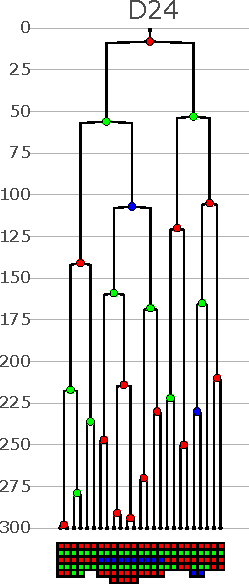
\includegraphics[width=0.18\textwidth]{images/cellLineage.pdf}
	\end{center}
\vspace{-20pt}
\caption[Colour-coded lineage tree.]{\bf Lineage tree.}
\vspace{-10pt}
\label{fig:cellLineage}
\end{wrapfigure}
%
We colour-coded the nodes in the lineage tree representation based on the corresponding division type to further analyse the division behaviour among several datasets (see Figure~\ref{fig:cellLineage}). The left labels show the time steps and an additional one at the top of each tree displays the total number of divisions. The colour of the nodes indicates the kind of division: \textcolor{red}{anticlinal}, \textcolor{green}{periclinal} and \textcolor{blue}{radial}. The ``bricks'' visualisation at the bottom of each tree allows a more adequate comparison of division sequences among several trees. The number of columns indicates the number of total leaf nodes while the rows in each column corresponds to the division type that each ``leaf cell'' has cycled through. For example, the outermost left leaf cell in the tree in Figure~\ref{fig:cellLineage} originated from an anticlinal, periclinal, anticlinal, periclinal and finally an anticlinal division. This sequence corresponds to the outermost left column of the bricks visualisation read from top to bottom. A visualisation of all cell lineages of all five datasets is given in Figure~\ref{fig:allTrees} and only the lineages located in the master cell files are illustrated in Figure~\ref{fig:allMasterTrees}.

\subsubsection{Periclinal Division Sequences}
\label{sec:treeDivisionSequence}
\noindent
Periclinal divisions are responsible for the layer organisations in the lateral root. We generated a division sequence tree to focus on these periclinal divisions (see Figure~\ref{fig:treeDivisionSequenceSample}).
%
\begin{figure}[htbp]
	\begin{center}
		\begin{overpic}[width=0.8\linewidth]{images/treeDivisionSequenceSample.pdf}
		\end{overpic}
\caption[Division sequence tree.]
{
{\bf Division sequence tree for dataset $\#120830$.}
}
	\label{fig:treeDivisionSequenceSample}
	\end{center}
\end{figure}
%
Through this, we are able to analyse the temporal layer organisation in a dataset and can compare it with other datasets. The layer assignment is given by a unique sequence (colour) and each dataset starts in a single layer (\textbf{0}). When a cell performs a periclinal division, its daughter cells are assigned to an outer (initially \textbf{01}) and an inner layer (initially \textbf{02}) with further layer generations in later time steps. This spatial layer organisation is rendered along the number of time steps. By this, we can easily detect when new layers are generated resulting in the identification of the high-order pattern of periclinal divisions for each dataset. The division sequence trees for all datasets are shown in Figure~\ref{fig:treeDivisionSequences}. The visualisation of the lineage trees as well as the division sequence trees are done in \textit{scifer}.

\clearpage
\section{Quantification and Visualisation of Deformation in the Virtual Lateral Root}
\noindent
The analysis of the temporal deformation information during the growth of the lateral root is inspired by the work of Graner~et~al.~\cite{graner_et_al_2008}. The idea is that the deformation can be computed using geometrical and topological properties of the underlying tissue. Since in our case we have a set of 3D cell nuclei for each time step (red nodes in Figure~\ref{fig:deformation}) we use this one to generate a triangulation (e.g. Delaunay triangulation) creating a surface that represents the tissue (see Figure~\ref{fig:deformation}). The deformation analysis can now be performed object- or spatial-oriented. This means that either the deformation is evaluated and illustrated for each cell or the total area of interest is subdivided into regions of equal sizes to measure the deformation within each of such a region. We consider the former case because we want to focus on individual cell changes. Besides, the number of cells are quite small at the beginning of our datasets so the total area of interest is not covered by all cells which makes an object-oriented analysis per cell more reasonable.
%
\begin{figure}[htbp]
	\begin{center}
		\begin{overpic}[width=1.\linewidth]{images/deformation.pdf}
		\end{overpic}
\caption[Surface generation for deformation analysis.]
{
{\bf Surface generation for deformation analysis.}
}
	\label{fig:deformation}
	\end{center}
\end{figure}
%

\subsection{Computation of Geometrical and Topological Contributions}
\noindent
The generation of a triangulation results in a neighbourhood information for each nuclei and we can further analyse how a cell deforms over time. Let $c_1$ be one cell with a position $p_{c_1} = ( x_1, y_1, z_1 )^T$. Another cell $c_2$ with position $p_{c_2} = ( x_2, y_2, z_2 )^T$ is a neighbour of $c_1$ if both share an edge or link $l = p_{c_2} - p_{c_1}$. Note that $l$ and $-l$ represent the same physical role but to be invariant under the change $l \rightarrow -l$, a so-called \textit{link matrix} $m$ is introduced~\cite{graner_et_al_2008}:
\begin{equation}
m = l \otimes l =
\begin{pmatrix}
X^2 & XY & XZ\\
YX & Y^2 & YZ\\
ZX & ZY & Z^2
\end{pmatrix}
, \qquad
\left( X, Y, Z \right) = \left( x_2 - x_1, y_2 - y_1, z_2 - z_1 \right).
\end{equation}
This matrix incorporates the square link length and the angle by computing the tensor product of the link $l$. The further computations consider the average of all relevant links $N$ for a specific cell which is defined as the \textit{texture tensor}~\cite{aubouy_et_al_2003}:
\begin{equation}
M = \langle m \rangle = \langle l \otimes l \rangle = 
\begin{pmatrix}
\langle X^2 \rangle & \langle XY \rangle& \langle XZ \rangle\\
\langle YX \rangle & \langle Y^2 \rangle & \langle YZ \rangle\\
\langle ZX \rangle & \langle ZY \rangle & \langle Z^2 \rangle
\end{pmatrix}
= \mathlarger{\mathlarger{\nicefrac{\sum\limits_{N} l \otimes l}{N}}}.
\end{equation}
%
\begin{figure}[htbp]
	\begin{center}
		\begin{overpic}[width=1.\linewidth]{images/ellipseDeformation.pdf}
		\end{overpic}
\caption[Deformation computation and representation.]
{
{\bf Left:} 2D example of \textcolor{blue}{conserved}, \textcolor{red}{appearing} and \textcolor{green}{disappearing} links between two time steps due two a cell division. {\bf Right:} Deformation is represented by the axes of an ellipse.
}
	\label{fig:ellipseDeformation}
	\end{center}
\end{figure}
%

\noindent
The geometrical and topological terms are now computed by considering the variation of conserved, appearing and disappearing links between two time steps $t$ and $t + \Delta t$ (see Figure~\ref{fig:ellipseDeformation}, left). More precisely, the geometrical variation, denoted as $B$ is computed by averaging the amount of conserved links $N_c$ between two time steps~\cite{graner_et_al_2008}:
\begin{equation}
B = \frac{N_c}{N} \left\langle \frac{\Delta m}{\Delta t} \right\rangle = \frac{N_c}{N} \left\langle \frac{\Delta (l \otimes l) }{\Delta t} \right\rangle.
\end{equation}
This means that $M$ is evaluated at $t$ and $t + \Delta t$ and the difference is computed. For small $\Delta t$ values, $\frac{N_c}{N} \rightarrow 1$ because then almost all of the total links $N$ are conserved and $B$ can then be written as:
\begin{equation}
B = \left\langle l \otimes \frac{dl}{dt} \right\rangle + \left\langle \frac{dl}{dt} \otimes l \right\rangle.
\end{equation}
The topological variation $T$ takes the averaging of the $N_a$ appeared and $N_d$ disappeared links into account depending on the corresponding averaged textures $\langle m_a \rangle$ and $\langle m_d \rangle$~\cite{graner_et_al_2008}:
\begin{equation}
T = \frac{1}{\Delta t} \left( \frac{\Delta N_a}{N} \langle m_a \rangle - \frac{\Delta N_d}{N} \langle m_d \rangle \right).
\end{equation}
The total deformation for each cell is then given by $B+T$. This sum is a matrix for which the eigenvalues $\lambda_i$ are computed. The magnitudes of these eigenvalues are proportional to the axes lengths of an ellipsoid that represents the spatial 3D deformation of a cell between $t$ and $t + \Delta t$ (see Figure~\ref{fig:ellipseDeformation}, right for a 2D case). We compute the $B$ and $T$ terms for all 3D cell positions but we focus the visualisation on the 2D views using the side (along shoot/root axis), front (growth towards the observer) and radial views (transversal cut perpendicular to shoot/root axis). Because of these 2D projections we illustrate the deformations by ellipses instead of ellipsoids in 3D for a more reasonable analysis. Figure~\ref{fig:ellipseResults} shows ellipses indicating the longest deformations of two datasets for the variation right before the last time step.
%
\begin{figure}[htbp]
	\begin{center}
		\begin{overpic}[width=1.\linewidth]{images/ellipseResults.pdf}
		\end{overpic}
\caption[Illustration of longest deformations by ellipses in two datasets in side view.]
{
{\bf Illustration of longest deformations by ellipses in two datasets in side view.}
}
	\label{fig:ellipseResults}
	\end{center}
\end{figure}
%

\subsection{Averaging over datasets}
\noindent
The above evaluation allows us to analyse the deformation of individual cells between two time steps $t$ and $t + \Delta t$. Our intention is to analyse the averaged deformation of the virtual lateral root with respect to all five datasets. This means that we require a spatial and a temporal registration of all datasets in such a way that the combined deformation information (i.e.~the ellipses) can be evaluated.

In order to apply a spatial registration, we compute the centre of mass, the principal components and the convex hull of the set of all 3D cell positions at the last time step. Our aim is that the convex hulls of different datasets should match optimally. Using this information each dataset is then initially translated to the origin (black node in Figure~\ref{fig:spatialRegistration}, top) according to the centre of mass and rotated by its associated principal components (arrows in Figure~\ref{fig:spatialRegistration}, top). Through this, we generate our three viewing types (front, side and radial) of the data which are almost similar among different lateral roots. Last refinements are done manually by slight affine transformations in such a way that the datasets fit to the base of the VLR with respect to the convex hulls (see Figure~\ref{fig:spatialRegistration}, bottom). This fitting represents an optimal basis for comparing different lateral roots developing from almost the same base position.

We perform a temporal registration based on the number of cells. For this purpose, the intersection set of the number of cells among all datasets for the first and last time steps are observed. So, the number of cells are in the range of $[10,176]$ for $\# 120830$, $[15,160]$ for $\# 121204$, $[18,260]$ for $\# 121211$, $[9,143]$ for $\# 130508$ and $[15,267]$ for $\# 130607$. Consequently, the intersection range is $[18, 143]$. With this, the time step size $\Delta t$ is actually the variation of number of cells depending on the total number of considered steps $S$:
\begin{equation}
\Delta t = \frac{143 - 18}{S},
\end{equation}
and the current number of cell $s(i)$ for each step $i$ is:
\begin{equation}
s(i) = \left\lfloor s_i + 0.5 \right\rfloor, \qquad s_i = s_{i-1} + \Delta t, \qquad s_0 = 18.
\end{equation}
The usage of the floor function performs a rounding of $s(i)$ to the nearest integer value because $\Delta t$ might be a float value. However, it cannot be guaranteed that $s(i)$ appears in each dataset because of several cell divisions at one time step. We solve this issue by determining the nearest smallest possible cell number with respect to the current $s(i)$.
%
\begin{figure}[htbp]
	\begin{center}
		\begin{overpic}[width=1.\linewidth]{images/spatialRegistration.pdf}
		\end{overpic}
\caption[Spatial registration of datasets.]
{
{\bf Top:} Generation of front, side and radial views according to centre of mass (black node) and principal components. {\bf Bottom:} Manual fitting based on convex hulls of datasets: \textcolor{magenta}{$\#120830$}, \textcolor{yellow}{$\#121204$}, \textcolor{red}{$\#121211$}, \textcolor{green}{$\#130508$}, \textcolor{blue}{$\#130607$}.
}
	\label{fig:spatialRegistration}
	\end{center}
\end{figure}
%

For each number of cell pair $s(i)$ and $s(i+1)$, $B+T$ is evaluated for each dataset resulting in the corresponding deformation information. To average it over all datasets we create a grid of tiles with constant but arbitrarily dimension (see Figure~\ref{fig:gridDeformation}, left). For each tile in the grid we compute the average deformation of all ellipses whose centres are located in the corresponding tile. More precisely, the deformation in 3D given by all three axes of the ellipsoid is first averaged for each cell. Let $d_1, d_2, d_3$ be the three deformation vectors and $m_1, m_2, m_3$ the corresponding magnitudes. The average deformation $d_a$ and average magnitude $m_a$ per cell is then given by the mean:
\begin{equation}
d_a = \frac{1}{3} \sum_{i=1}^{3} d_i, \qquad m_a = \frac{1}{3} \sum_{i=1}^{3} m_i.
\end{equation}
Afterwards, the deformation vectors $d_a$ and the corresponding magnitudes $m_a$ of all $n$ cells located in the same tile are averaged:
\begin{equation}
D_a = \frac{1}{n} \sum_{n} d_a, \qquad M_a = \frac{1}{n} \sum_{n} m_a.
\end{equation}
Through this, each tile represents an averaged deformation that is represented by a line with normalized length. The averaged magnitudes are illustrated by a colour map and additional ``bow ties'' illustrate the variance of the deformation orientation (see Figure~\ref{fig:gridDeformation}, right).
%
\begin{figure}[htbp]
	\begin{center}
		\begin{overpic}[width=1.\linewidth]{images/gridDeformation.pdf}
		\put(44.5,10.5){\small low}
		\put(55.1,10.5){\small high}
		\end{overpic}
\caption[Averaging over datasets and visualisation of deformation information.]
{
{\bf Left:} Example of how the deformation information of all datasets is averaged using a grid approach. {\bf Right:} Visualisation of averaged deformation information by colour-coded lines according to magnitude values given in Table~\ref{tab:deformationParameters} and ``bow ties'' over all datasets in side view. The contour shows the convex hull using a B\'ezier curve.
}
	\label{fig:gridDeformation}
	\end{center}
\end{figure}
%

We perform this averaging for all three viewing types (front, side, radial). Figure 2B in the main manuscript shows the deformation result for the first, mid and last time step ranges. For the front and radial view, we illustrate the deformation for all cells while for the side view we focus only one the cell changes located in the master cell file. Note that we determine in all cases the deformation information based on all 3D+t cell data. Table~\ref{tab:deformationParameters} lists the minimum and maximum magnitudes for the deformations according to the different viewing types. We have chosen $S=20$ steps for which $\Delta t = 6.25$ with an average increasing rate by $12.06$ cells per step. The deformation computation as well as the visualisation are realized using \textit{MATLAB} (\href{http://www.mathworks.com/products/matlab/}{http://www.mathworks.com/products/matlab/}). \TODO{add the exact number of considered cells for each step to the movie description.}

\clearpage
\section{Modelling}
\TODO{\@ JENS: as we are never using the results of the data-driven models, I wonder whether the triangle mesh section should even appear. It could appear confusing. What do you think?}
\noindent
Our non-mechanical 2D modelling approach of the VLR development is based on L-systems or also called Lindenmayer~Systems~\cite{lindenmayer_1968, prusinkiewicz_lindenmayer_1990}. The L-system is a language that consists of a set of strings based on predefined rules. More precisely, it consists of an axiom, the starting point of the system, and a set of production rules. The growth of a dynamic structure is realized by applying these rules to the axiom in which the resulting string is again in the language of the used system. Through this, the growth can be described by an infinite set of strings that 'steers' the growth behaviour. L-systems are commonly used to model plant growths as well as to generate fractals such as the Sierpinski triangle, for example.

We are using a 2D model for two reasons. First, such a model is much easier to describe than in 3D which significantly reduces the model complexity. Second, we can focus on the 2D case because we want to compare the model result with the real-world cells located in the master cell file of the VLR. These cells feature the property that their positions almost lie on a plane in 3D and that they can be projected onto a 2D plane in side view. Furthermore, based on our analysis the cells in the master cell file are the main contributor to the data-driven growth of the VLR.

The evolving 2D tissue of the model can be described by a graph, i.e.~an abstract structure in which a set of vertices is connected by a set of edges. In the context of cell representation, an edge denotes a cell wall and a vertex corresponds to a junction that forms the meeting point of at least two cell walls~\cite{prusinkiewicz_lindenmayer_1990, prusinkiewicz_runions_2012}. As a consequence, the complete topology of all cells in the tissue model such as neighbourhood information can be accessed via a graph rotation system~\cite{edmonds_1960}. We realize the implementation of such a model using \textit{OpenGL} (\href{https://www.opengl.org/}{https://www.opengl.org/}) and the \textit{VV} (Vertex-Vertex) programming language~\cite{smith_et_al_2004, smith_2006} which is embedded in a C{}\verb!++! programming environment.

\noindent
Our modelling approach has the following requirements which are explained in detail in the sections below:
\begin{Itemize}
\item \textbf{Model Surface:} The model requires an underlying surface structure that represents the developing VLR.
\item \textbf{Founder Cells:} Additionally, the positioning and the number of founder cells that contribute to the VLR have to be determined.
\item \textbf{Division Properties:} The behaviour of a cell division event has to be defined, i.e.~what type of division and when should it take place.
\end{Itemize}

In a nutshell, the simulation starts with a specific number and positioning of founder cells and develops over time based on the underlying surface structure. During the simulation, the VLR and the cells within grow and increase in area size. According to the chosen division properties, a cell will divide if it exceeds a specific area threshold or area ratio with respect to its initial size right after its birth. Through this, we can generate a convenient model representing the growth of the VLR.

\subsection{Model Surfaces}
\noindent
The choice of the underlying surface for the model fundamentally affects the development of the tissue. This means that the changing vertices of the surface influence the evolving cells of the model and their corresponding walls and junctions. We use two surface types to represent the structure of the VLR: Triangle meshes and B\'ezier surfaces. The first one is used to create a triangulation based on real nuclei positions in the dataset for each time step. Through this, we can generate a data-driven model that incorporates the deformation behaviour of the nuclei and are able to compare the result with the real-world datasets. The B\'ezier surface is used for a generalized model that allows an investigation of a common growth behaviour of the VLR. For this, we use non-deterministic division rules for each model, i.e.\ a random variation of the division line orientation which is explained below in section~\ref{sec:divisionRules}. By running such a slight random model with the same setting several times (e.g.\ 100) we can analyse its division behaviour based on statistically solid results.

\subsubsection{Triangle Mesh}
\noindent
For each real-world dataset, we create a set of 2D triangle meshes. This means that for each time step, we generate a triangulation based on the corresponding real nuclei positions located in the master cell file only because these are mainly responsible for the overall dome-like structure of the VLR. Through this, the triangulation captures the temporal displacement and growth behaviour of the nuclei which is then further used in the model to dictate the simulation and tissue growth (see Figure~\ref{fig:surfaceGeneration}). More precisely, the cells in the model consists of changing junctions that are affected by the triangle changes. If a junction $j$ of a cell is located within a specific triangle then $j$ is given uniquely by a convex combination $j = \lambda_1 r_1 + \lambda_2 r_2 + \lambda_3 r_3$ of the three triangle vertices $r_i$. The $\lambda_i$ $\left( \sum_{i=1}^{3} \lambda_i = 1, \lambda_i \geq 0 \; \forall i \right)$ are called the barycentric coordinates of $j$ with respect to the triangle. In the model itself, a lot of conversions between these barycentric and Cartesian coordinates occur to compute the changing cells.
%
\begin{figure}[htbp]
	\begin{center}
		\begin{overpic}[width=1.\linewidth]{images/surfaceGeneration.pdf}
		\end{overpic}
\caption[Generation of triangle mesh based on real nuclei displacements.]
{
{\bf Generation of triangle mesh based on real nuclei displacements.}
}
	\label{fig:surfaceGeneration}
	\end{center}
\end{figure}
%

The triangulation can be either realized by a Delaunay triangulation or an $\alpha$-shape. Since we are only using the nuclei to construct the triangulation we require some additional information to of the VLR contour. Therefore, for each dataset, we manually generate a set of contour points to approximate the boundary of the VLR for the first (bottom left image in Figure~\ref{fig:surfaceGeneration}) and the last (bottom right image in Figure~\ref{fig:surfaceGeneration}) time step. We choose a constant number of 16 points such that the contour points for the time steps in between are interpolated linearly (see bottom mid image in Figure~\ref{fig:surfaceGeneration}).
%
\begin{figure}[htbp]
	\begin{center}
		\begin{overpic}[width=0.8\linewidth]{images/surfaceMapping.pdf}
%			\putIndex{0}{0}{A.pdf}
%			\putIndex{52}{0}{B.pdf}
		\end{overpic}
\caption[Mapping of triangles and nuclei between subsequent time steps.]
{
{\bf Mapping of triangles and nuclei between subsequent time steps.} Nuclei displacements only do not interfere the bijectivity requirement but cell divisions do result in more triangles.
}
	\label{fig:surfaceMapping}
	\end{center}
\end{figure}
%

For the set of generated meshes, a bijective mapping of the triangles between time step $t$ and $t+1$ is required for the computation of arbitrary cell positions in between in the model. This means that each nuclei position in time step $t+1$ is uniquely assigned to a previous position in time step $t$ (top left in Figure~\ref{fig:surfaceMapping}). More precisely, our approach requires that we use the same triangulation (but with different nuclei positions) for subsequent time steps. However, cell divisions may result in more nuclei in the next time step and consequently in more triangles (top right in Figure~\ref{fig:surfaceMapping}) impairing the bijectivity. To overcome this issue, for each occurring cell division, the average position of the two daughter cells (grey nodes) is computed at the next time step and represents a single nuclei position (cyan node) that can be bijectively mapped to the previous dividing cell (green node). At time step $t+2$, the two triangles originally created at $t+1$ are considered and the next time step $t+3$ is checked again. In total, there are two triangle meshes for each pair of subsequent time steps that guarantee a bijective mapping which are between time step $t$ and $t+1$, as well as $t+2$ and $t+3$, respectively.

The exchange of the different triangle meshes between $t+1$ and $t+2$ is realized by another approach. Consider the simplified model with three cells in Figure~\ref{fig:triangleExchange} and the inner junction $j$ in the model. At time step $t$, the position of $j$ is computed by its barycentric coordinates within the blue-rimmed triangle. When in the next time step the triangle mesh should have changed then it will be checked in which triangle $j$ is located now. Based on the position in the newly found blue-rimmed triangle, the new barycentric coordinates are computed. In further steps, either only a bijective mapping between two equal triangulations is needed or the same approach is applied facing a new triangle mesh. Note that at the beginning of the model, the setting of cells as well as their positions have to be defined manually. Based on these positions, the triangles are identified in which the junctions are located and the barycentric coordinates are computed.
%
\begin{figure}[htbp]
	\begin{center}
		\begin{overpic}[width=0.8\linewidth]{images/triangleExchange.pdf}
%			\putIndex{0}{0}{A.pdf}
%			\putIndex{52}{0}{B.pdf}
		\end{overpic}
\caption[Transition between two different triangle meshes.]
{
{\bf Transition between two different triangle meshes.} For each junction position $j$, the triangle of the underlying surface has to be identified in which $j$ is located at time step $t+1$. The red nodes indicate the nuclei while the black ones denote the contour points.
}
	\label{fig:triangleExchange}
	\end{center}
\end{figure}
%

\subsubsection{B\'ezier Surface}
For this idealized model, we use a set of B\'ezier surfaces to represent the smooth tissue development. A two-dimensional B\'ezier surface of degree $(n, m)$ with $(n+1) \cdot (m+1)$ control points $c_{i, j} \in \mathbb{R}^2$ is a parametric surface that maps the unit square into a smooth-continuous surface embedded in the same space as its control points. Each point $P(u, v) \in \mathbb{R}^2$ on such a B\'ezier surface $S_{cur}$ with parametric coordinates $u ,v \in [0,1]$ is computed by the following equation:
\begin{equation}
P(u, v) = \sum_{i=0}^{n} \sum_{j=0}^{m} B_{i}^{n} (u) \; B_{j}^{m} (v) \; c_{i,j}, \qquad B_{i}^{n} (u) = \binom{n}{i} u^i (1-u)^{n-i}.
\end{equation}
As a consequence, given only an initial surface $S_{init}$ and a final B\'ezier surface $S_{final}$ to describe the first and the last time step of the model, the surface at each other time step in between is computed by a linear interpolation of the control points $a_{i,j} \in S_{init}$ and $b_{i,j} \in S_{final}$:
\begin{equation}
c_{i,j} = (1-t) \cdot a_{i,j} + t \cdot b_{i,j}, \qquad \forall i, j \in [0, n], [0, m],
\end{equation}
with the control points $c_{i,j} \in S_{cur}$ and $t \in [0,1]$ as the temporal interpolation factor. Through this, only two B\'ezier surfaces need to be generated manually for the model while the remaining ones are given by interpolation which ensures a smooth growth behaviour of the VLR. Another advantage of using this kind of surface is that the mapping of each pair of parametric coordinates $u_i, v_i$ to a 2D position on the surface is unique although of course the developing surface structure will change over time (see Figure~\ref{fig:modelSurface}).
%
\begin{figure}[htbp]
	\begin{center}
		\begin{overpic}[width=0.8\linewidth]{images/modelSurface.pdf}
		\end{overpic}
\caption[Initial and final B\'ezier surface of degree $(6, 6)$ for the generalized model.]
{
{\bf Initial and final B\'ezier surface of degree $(6, 6)$ for the generalized model.} The mapping of $(u_i, v_i)$ to the changing position on the surface is unique over time.
}
	\label{fig:modelSurface}
	\end{center}
\end{figure}
%

\subsection{Setting of Founder Cells}
\noindent
For the modelling approach we have to set the number and spatial properties of founder cells that affect the overall development of the lateral root. We are using two different setting types depending on the kind of model.

\subsubsection{Data-driven Models}
\noindent
The first setting is designed in such a way that a valid comparison between model and real world dataset is achieved. The underlying surface of the model is a triangle mesh based on real nuclei positions as explained above. Furthermore, the number of cells in the model is selected such that it approximately matches the same number of cells in the real-world datasets for both, the beginning and the end of the given datasets. In order to preserve the same number of cells at the end in the model, we steer the parameter for the division event as explained later.

\subsubsection{Idealized Models}
\noindent
For the generalized model, we use a B\'ezier surface starting with two founder cells sharing the same size and shape (see Figure~\ref{fig:founderCellsSetting}, left). We consider three different division settings at the beginning. In the first one, the model starts with two founder cells sharing the same size and the tissue further develops depending on the selected division rules explained below. In another setting, the model starts identically but we hardwire the first division cycle with an anticlinal division (see Figure~\ref{fig:founderCellsSetting}, middle). More precisely, the inner daughter cells share the same size but with only one third of the parents cell's size. In the last scenario, we additionally hardwire the second division cycle simulating a periclinal division behavior (see Figure~\ref{fig:founderCellsSetting}, right). Note that the interphase durations between the division cycles take some steps in the model in which the overall lateral root already started to evolve and eventually changed its tissue structure. But for the sake of clarity, the three surface tissues in Figure~\ref{fig:founderCellsSetting} are the same. \TODO{add naming convention for each hardwired situation.}
\TODO{Harmonize naming with the one of main text/figure (a minima: explaining the equivalence between the naming in the main text/figure and what you name here.}
%
\begin{figure}[htbp]
	\begin{center}
		\begin{overpic}[width=1.\linewidth]{images/founderCellsSetting.pdf}
%			\putIndex{0}{0}{A.pdf}
%			\putIndex{52}{0}{B.pdf}
		\end{overpic}
\caption[Initial situation of founder cells in the generalized model and hardwired division cycles.]
{
{\bf Initial situation of founder cells in the generalized model and hardwired division cycles.} \TODO{add 2DCBase}
}
	\label{fig:founderCellsSetting}
	\end{center}
\end{figure}
%

\subsection{Division Properties}
\noindent
The division behaviour is a fundamental property of the tissue model to evolve. For this purpose, it has to be determined when a cell division should occur and how the division line has to be set that splits the cell into two daughter cells.

\subsubsection{Division Event}
\noindent
For each cell in the model the initial area size is computed that a cell has right after its birth. In each model step, the current area of each cell is computed and compared with its initial area size. If the cell's area exceeds the initial area by a certain amount then a division event will occur. This amount is determined in using an \textit{area ratio} as well as an \textit{area threshold}. The first parameter allows the user to set up the percentage expansion of a cell. For example, a ratio of $0.5$ denotes that the cell will divide if its initial size has increased by at least $50\%$. However, only using this ratio would result in cell sizes that converge to zero in later steps. For this reason, the area threshold is used as a barrier to guarantee a minimum area size for each cell before it divides.

\subsubsection{Division Rules}
\label{sec:divisionRules}
\TODO{Harmonize naming with the one of main text/figure (a minima: explaining the equivalence between the naming in the main text/figure and what you name here.}
\noindent
After defining the occurrence of a division event we need to set the orientation of the division line. In our model approach we consider five different division scenarios (see Figure~\ref{fig:divisionRules}):
\begin{Itemize}
\item Besson-Dumais (BD),
\item Decussation (D) + random variation,
\item Perpendicular to principal direction of growth (PDG) + random variation,
\item Random (R) and,
\item Random with equal daughter cell sizes (RE).
\end{Itemize}
%
\begin{figure}[htbp]
	\begin{center}
		\begin{overpic}[width=1.\linewidth]{images/divisionRules.pdf}
		\end{overpic}
\caption[Division scenarios used in our modelling approach.]
{
{\bf Division scenarios used in our modelling approach.}
}
	\label{fig:divisionRules}
	\end{center}
\end{figure}
%

The Besson-Dumais \textbf{(BD)} division rule~\cite{besson_and_dumais_2011} can be seen as a generalization of the shortest wall or Errera's rule~\cite{errera_1886} which will always result in the shortest division line that can be generated to connect two opposing cell walls through the centre of mass (red dots in Figure~\ref{fig:divisionRules}). Using BD, each line orientation of a set of $N$ possible orientations is assigned a specific probability value based on the length $l_i$ of the line and the cell's area:
\begin{equation}
p_i = \frac{e^{-\beta l_i / \rho}}{\sum_{j=1}^{N} e^{-\beta l_j / \rho}}.
\end{equation}
$\rho = \sqrt{A}$ is the mean cell diameter and $\beta = 20.6$ is a parameter that was measured experimentally by Besson and Dumais~\cite{besson_and_dumais_2011} for which the proportion of cells dividing along the shortest wall is supported by this value. As a consequence, we have a probability distribution function for the set of division lines and the line with the highest probability is identical with the shortest one. Figure~\ref{fig:divisionRules},BD illustrates three examples of division orientations and their corresponding colour-coded probabilities.

The next scenario is in choosing a division line that is perpendicular to the principal direction of the cell's growth \textbf{(PDG)}. More precisely, for one cell from the time since its birth until the time it will divide, the principal component for the set of changing centre of mass positions is computed. The new division line is then perpendicular to this direction. This means that the whole division behaviour is deterministic when using this rule only. But in order to compare it with the BD rule which is in fact a probability distribution, we allow a small randomized variation of the division orientation which is denoted by $\alpha$ (e.g. $10$). More in detail, after determining the new division line, its orientation can still be varied by an angle of $\pm \; \alpha$ (see Figure~\ref{fig:divisionRules}, PDG).

The decussation rule \textbf{(D)} will result in a division line that is always perpendicular to the previous division line of the parent cell. The initial division line orientation is given by the setting of the founder cells. Thus, also using this rule is deterministic and we consider also here a randomized variation of the division line given by $\alpha$ (see Figure~\ref{fig:divisionRules}, D). Note that the interphase between these two division events take some time in which the cell's size is increasing. However, in Figure~\ref{fig:divisionRules}, D, the cell has the same size and shape in the next division cycle for the sake of clarity.

The random rule \textbf{(R)} generates arbitrary division line orientations through the centre of mass with respect to a cell-shape preserving property that is explained below. All possible division orientations have the same probability.

The last scenario is considering a random rule but preserving almost equal area sizes of the daughter cells \textbf{(RE)}. Note that when using only straight lines as division walls a perfect splitting of a cell into two equal areas is not always satisfied. As a consequence, it cannot be guaranteed that the division line is in a right angle to both connected cell walls. But for simplification in the model analysis we stick to not a curved division line but only a straight one.

%
\begin{figure}[htbp]
	\begin{center}
		\begin{overpic}[width=0.8\linewidth]{images/shapePreserving.pdf}
		\end{overpic}
\caption[Cell Shape Preservation.]
{
{\bf Cell Shape Preservation.} For each division line through the centre of mass rotated by an user-selected angle $\alpha$, a length check of the connected cell walls is applied. For this purpose, the two interconnection nodes $u$ and $v$ as well as the adjacent junctions $u_1, u_2$ and $v_1, v_2$ are determined. From these positions the lengths $a, b, c, d$ and the cell wall lengths $a+b$ and $c+d$ are computed. It is now checked in four cases if $a < (a+b)\cdot \delta$, $b < (a+b)\cdot \delta$, $c < (c+d)\cdot \delta$, or $d < (c+d)\cdot \delta$. If only one statement is false then this division line orientation is omitted. The user-selected value $\delta$ is in $[0,1]$ and denotes the percentage that a sub-line must have with respect to the total call wall length.
}
	\label{fig:shapePreserving}
	\end{center}
\end{figure}
%

\subsubsection{Cell Shape Preservation}
\noindent
In the model, a total random configuration of cell division lines may result in implausible cell developments with unequal sizes and triangle-shaped contours that cannot be observed in any real-world scenario of plant growth. However, we want to analyse a random behaviour of cell divisions that somehow preserve equal sizes and shapes of cells while dividing. We therefore first find a set of division line orientations that satisfy a specific constraint and assign each one the same probability value. The idea of this approach is explained in Figure~\ref{fig:shapePreserving}. We use a value of $\delta = 0.15$ for the division rule R and RE while this value is set to zero for BD, D and PDG.

\subsubsection{Modified Computation of Centre of Mass.}
\noindent
Remark that for all division rules the division line passes always through the centre of mass. However, in later model steps, morel cells are created that share several junctions (see Figure~\ref{fig:levelOfDetail}, left).
%
\begin{figure}[htbp]
	\begin{center}
		\begin{overpic}[width=1.\linewidth]{images/levelOfDetail.pdf}
		\end{overpic}
\caption[Modified computation of centre of mass.]
{
{\bf Modified computation of centre of mass. Left:} The centre of mass of cells with several junctions may not yield a ``real'' centre of the cell. \textbf{Right:} Using a level of detail approach yields few junctions preserving the shape of the cell.
}
	\label{fig:levelOfDetail}
	\end{center}
\end{figure}
%
Consequently, a cell consists of more junctions and the computed centre of mass will be located near the mass of junctions (blue node in Figure~\ref{fig:levelOfDetail}, left). This may result in an implausible division line that also does not preserve equal areas of daughter cells. In order to solve this issue, we perform a \textit{level of detail} of cell walls called the \textit{edge criterion} in such a way that only these junctions are preserved that mainly captures the shape of the cell. For example, the cell in Figure~\ref{fig:levelOfDetail} has seven junctions. Performing a level of detail results in a simplified cell shape that only has four junctions left (see Figure~\ref{fig:levelOfDetail}, right) while preserving the main shape structure of the cell. The centre of mass is then computed based on these remaining junctions. A detailed description of the algorithm can be found in \cite[p.\ 59--60]{FangerauDiss_2015}. Note that we apply this level of detail only for the computation of the centre of mass. We do not remove any junctions of cells in the model itself.

\subsubsection{Parameter Setting for Data-driven and Idealized Models}
\noindent
For each model setting we perform $100$ runs with $500$ steps to test how stable the model and therefore the divisions results are based on the randomized factor included in each division rule. Furthermore, we use a constant area threshold value of $1100$ while the area ratio is steered in such a way that at the end of each model step a certain number of cells is reached. For the data-driven models, this number is chosen to be almost identical to the number of cells in the master cell file of the real-world datasets. For the idealized models, we tried to set an area ratio value in such a way that at the end approximately $64$. This value is chosen based on the average number of cells in the master cell file for all five wild type datasets ($(64+49+81+45+82)/5 \approx 64$). The comprehensive Table~\ref{tab:modelParameters} lists all area ratios, average number of cells, anticlinal and periclinal divisions for both the data-driven and the idealized models for each hard-wired division setting that is analysed.

\subsection{Visual Analysis of Models}
\subsubsection{Visualisation Approaches}
\noindent
For each model setting, we generate three different representations of the evolving cells in the tissue: Illustration of
\begin{inparaenum}[(\itshape A\upshape)]
\item all cell contours (see Figure~\ref{fig:modelVisualisation}, left),
\item cells as spheres (see Figure~\ref{fig:modelVisualisation}, mid),
\item adjacent cell layers (see Figure~\ref{fig:modelVisualisation}, right).
\end{inparaenum}
%
\begin{figure}[htbp]
	\begin{center}
		\begin{overpic}[width=1.\linewidth]{images/modelVisualisation.pdf}
		\end{overpic}
\caption[Representation of evolving cells in model.]
{
{\bf Representation of evolving cells in model.} The model result can be illustrated by cell contours, cell spheres or by cell layers.
}
	\label{fig:modelVisualisation}
	\end{center}
\end{figure}
%
The first representation shows all cell contour information within the evolving tissue. Each cell is coloured by a gradient with focus on the computed centre of mass. The positions of the rendered spheres are given by the centres of mass of each cell. The third representation displays the cell layers between adjacent cells that share the same layer value (colour). Cells are adjacent if they share at least one common cell wall. The lines (cylinders) are drawn for at least two cells through the centres of mass of the corresponding cells.

\subsubsection{Division Analysis}
\noindent
We can run several samples of the model using division rules that include a randomized factor with each resulting in one division sequence tree as explained in section~\ref{sec:treeDivisionSequence}. However, we want to visually check how often and where the high-order pattern of periclinal divisions is preserved among several runs. This allows us to use statistically solid results of the model to compare them with the real-world datasets.
%
\begin{figure}[htbp]
	\begin{center}
		\begin{overpic}[width=0.4\linewidth]{images/averagedTreeDivisionSequence.pdf}
		\end{overpic}
\caption[Averaged division sequence tree.]
{
{\bf Averaged division sequence tree.} In only $48 \%$ of the $100$ comparisons in total, the upper layers were generated before the lower ones resulting in a red rectangle. In the other two cases with fewer comparisons ($81$ and $92$), more than $74 \%$ of the upper layers were generated first and green rectangles are drawn.
}
	\label{fig:averagedTreeDivisionSequence}
	\end{center}
\end{figure}
%
For this purpose, we modify the visualisation of the division sequence trees. Let $l$ be the sequence length for a generated layer (e.g.\ $l=3$ for $012$). We replace the x-axis showing the time steps by a fixed temporal layout of the tree in which the pair of upper concurrently generated layers (with identical number sequence except for the last number) always occur first (slight translation to the left) with respect to its lower layers with almost the same division sequence (except for the $(l-1)$-th number). For example, the pair of layers $0111/0112$ are combined because their sequence only differ in the last number. This pair is compared with the pair $0121/0122$ because they differ in the third ($l-1 = 4-1 = 3$) position of the sequence. For each such a comparison we render a rectangle that includes these two pairs of layers and is coloured by red or green. The rectangle is green if in more than $50 \%$ of the model samples the upper layer occurred first with respect to the lower one else it is red. This allows an immediate visual feedback of the high-order pattern while detailed information about the percentage and number of possible comparisons are given in the mid of each rectangle (see Figure~\ref{fig:averagedTreeDivisionSequence}). A comparison is not possible in a model when only one pair of layers is generated or none at all.

\subsubsection{Smoother Cell Contours}
\noindent
One initial cells consists of four junctions that define a rectangular cell shape within the underlying tissue.
%
\begin{figure}[htbp]
	\begin{center}
		\begin{overpic}[width=1.\linewidth]{images/subdivision.pdf}
		\end{overpic}
\caption[Subdivision approach for model tissue.]
{
{\bf Subdivision approach for model tissue. Top:} Using only six junctions (red nodes) for two cells result in a coarse tissue development based on the underlying B\'ezier surface. \textbf{Bottom:} Creating more inner junctions (cyan nodes) result in a much smoother tissue development.
}
	\label{fig:subdivision}
	\end{center}
\end{figure}
%
For example, consider the initial B\'ezier surface from Figure~\ref{fig:modelSurface} and having two cells at the first model step resulting in six junctions (two are shared by the cells) with their corresponding parametric coordinates (see Figure~\ref{fig:subdivision}, top left). In a later model step of the VLR, the tissue will start to grow evolving into the dome-like structure (see Figure~\ref{fig:subdivision}, top right). However, only the junction with the parametric coordinate $(u=\nicefrac{1}{2}, v=1)$ will move upwards based on the underlying B\'ezier surface creating a triangle-shaped tissue. In order to better approximate the underlying surface, additional inner junctions (cyan nodes in Figure~\ref{fig:subdivision}, bottom left) are created that result in a much smoother tissue development of the model (see Figure~\ref{fig:subdivision}, bottom right). This smoothness is defined by a user-chosen subdivision level which is $4$ in all our models and yields $2^{4-1} - 1 = 7$ additional inner junctions.

\clearpage
%%%%%%%%%%%%%%%%%%%%%%%%%%%%%%%%%%%%%%%%%%%%%%%%%%%%%%%%%%%%%%%%%%%%%%%%%%%%%%%%%%%%%%%%%%%%%%%%%%%%%%%%%%
% SUPP TABLES
%%%%%%%%%%%%%%%%%%%%%%%%%%%%%%%%%%%%%%%%%%%%%%%%%%%%%%%%%%%%%%%%%%%%%%%%%%%%%%%%%%%%%%%%%%%%%%%%%%%%%%%%%%
\section{Supporting Tables, Figures, Movies and Datasets}
\subsection{Supporting Tables}
\noindent
% Reset the Figure numbering and Add the "S"
\setcounter{table}{0}
\makeatletter 
\renewcommand{\thetable}{S\@arabic\c@table}
\makeatother
%
\TODO{fix format and floating}
% more space between rows
\renewcommand{\arraystretch}{1.2}
%
\begin{sidewaystable}\centering
\begin{tabular}{ | l | l | l | l | l | l | l | }
\hline
	Dataset & \#120830 & \#121204 & \#121211 & \#130508 & \#130607 & \#131203 \\ \hline
	Specimen & Arabidopsis thaliana, Col-0 & Arabidopsis thaliana, Col-0 & Arabidopsis thaliana, Col-0 & Arabidopsis thaliana, Col-0 & Arabidopsis thaliana, Col-0 & Arabidopsis thaliana, Col-0
aur1-2 aur2-2 double mutant \\ \hline
	Reporters & pGATA23::GUS-GFP-NLS & pGATA23::GUS-GFP-NLS & pGATA23::GUS-GFP-NLS & pGATA23::GUS-GFP-NLS & pGATA23::GUS-GFP-NLS & pUBI10::H2B-RFP \\ \hline
	 & pUBI10::H2B-RFP & pUBI10::H2B-RFP & pUBI10::H2B-RFP & pUBI10::H2B-RFP & pUBI10::H2B-RFP & pPIN1::PIN1-GFP \\ \hline
	 & pUBQ10::YFP-PIP1;4 & pUBQ10::YFP-PIP1;4 & pUBQ10::YFP-PIP1;4 & pUBQ10::YFP-PIP1;4 & pUBQ10::YFP-PIP1;4 & \ \\ \hline
	\ & \ & \ & \ & \ & \ & \ \\ \hline
	Growth & Cultivation Percival E-41L3 Plant Incubator & Cultivation Percival E-41L3 Plant Incubator & Cultivation Percival E-41L3 Plant Incubator & Cultivation Percival E-41L3 Plant Incubator & Cultivation Percival E-41L3 Plant Incubator & Cultivation Percival E-41L3 Plant Incubator \\ \hline
	Seeds Sowed: 23.8.2012 & Seeds Sowed: 26.11.2012 & Seeds Sowed: 5.12.2012 & Seeds Sowed: 2.5.2013 & Seeds Sowed: 31.5.2013 & Seeds Sowed: 26.11.2013 & \ \\ \hline
	1/2 MS Culture Medium Plates & 1/2 MS Culture Medium Plates & 1/2 MS Culture Medium Plates & 1/2 MS Culture Medium Plates & 1/2 MS Culture Medium Plates & 1/2 MS Culture Medium Plates & \ \\ \hline
	2.33 g/L MS (Duchefa, M0222.0050, LOT\# P08381.01) & 2.33 g/L MS (Duchefa, M0222.0050, LOT\# P08381.01) & 2.33 g/L MS (Duchefa, M0222.0050, LOT\# P08381.01) & 2.33 g/L MS (Duchefa, M0222.0050, LOT\# P08381.01) & 2.33 g/L MS (Duchefa, M0222.0050, LOT\# P08381.01) & 2.33 g/L MS (Duchefa, M0222.0050, LOT\# P08381.01) & \ \\ \hline
	1.5 \% Phytagel (Sigma, p8169-500G, LOT\# 048k0017) & 1.5 \% Phytagel (Sigma, p8169-500G, LOT\# 048k0017) & 1.5 \% Phytagel (Sigma, p8169-500G, LOT\# 048k0017) & 1.5 \% Phytagel (Sigma, p8169-500G, LOT\# 048k0017) & 1.5 \% Phytagel (Sigma, p8169-500G, LOT\# 048k0017) & 1.5 \% Phytagel (Sigma, p8169-500G, LOT\# 048k0017) & \ \\ \hline
	0.1\% MES (Sigma, M3671-50G, LOT\# 120M5433) & 0.1\% MES (Sigma, M3671-50G, LOT\# 120M5433) & 0.1\% MES (Sigma, M3671-50G, LOT\# 120M5433) & 0.1\% MES (Sigma, M3671-50G, LOT\# 120M5433) & 0.1\% MES (Sigma, M3671-50G, LOT\# 120M5433) & 0.1\% MES (Sigma, M3671-50G, LOT\# 120M5433) & \ \\ \hline
	1\% Saccharose (Roth, 4621.1, LOT\# 330160546) & 1\% Saccharose (Roth, 4621.1, LOT\# 330160546) & 1\% Saccharose (Roth, 4621.1, LOT\# 330160546) & 1\% Saccharose (Roth, 4621.1, LOT\# 330160546) & 1\% Saccharose (Roth, 4621.1, LOT\# 330160546) & 1\% Saccharose (Roth, 4621.1, LOT\# 330160546) & \ \\ \hline
	Growth Conditions & Growth Conditions & Growth Conditions & Growth Conditions & Growth Conditions & Growth Conditions & \ \\ \hline
	 & Light Intensity = 120-140 $\mu$mol*m-2*s-1 & Light Intensity = 120-140 $\mu$mol*m-2*s-3 & Light Intensity = 120-140 $\mu$mol*m-2*s-4 & Light Intensity = 120-140 $\mu$mol*m-2*s-5 & Light Intensity = 120-140 $\mu$mol*m-2*s-6 & Light Intensity = 120-140 $\mu$mol*m-2*s-6 \\ \hline
	Light Cycle Day/Night = 16/8 & Light = 16h Day, 8h Night & Light = 16h Day, 8h Night & Light = 16h Day, 8h Night & Light = 16h Day, 8h Night & Light = 16h Day, 8h Night & \ \\ \hline
	Temperature = 22\degree C & Temperature = 22\degree C & Temperature = 22\degree C & Temperature = 22\degree C & Temperature = 22\degree C & Temperature = 22\degree C & \ \\ \hline
	 & Gravistimulation Prior To Recording = 8h 34min & Gravistimulation Prior To Recording = 14h 20min & Gravistimulation Prior To Recording = 15h 45min & Gravistimulation Prior To Recording = 8h 25min & Gravistimulation Prior To Recording = 7h 15min & Gravistimulation Prior To Recording = 12h 40min \\ \hline
	 & 30.08.12, 7:50am - 16:00pm & 3.12.2012, 11:00pm - 9:00am (+1 Day) & 10.12.2012, 11:00pm - 9:00am (+1 Day) & 8.5.2013, 04:00am - 11:00am & 3.6.2013, 07:45am - 14:45pm & 3.12.2013, 00:00am - 07:30am \\ \hline
	 & & & & & & \ \\ \hline
	Light sheet Imaging & Cultivation in microscope & Cultivation in microscope & Cultivation in microscope & Cultivation in microscope & Cultivation in microscope & Cultivation in microscope \\ \hline
	Perfused Medium = 1/2 MS Medium & Perfused Medium = 1/2 MS Medium & Perfused Medium = 1/2 MS Medium & Perfused Medium = 1/2 MS Medium & Perfused Medium = 1/2 MS Medium & Perfused Medium = 1/2 MS Medium & \ \\ \hline
	 & 2.33 g/L MS (Duchefa, M0222.0050, LOT\# P08381.01) & 2.33 g/L MS (Duchefa, M0222.0050, LOT\# P08381.01) & 2.33 g/L MS (Duchefa, M0222.0050, LOT\# P08381.01) & 2.33 g/L MS (Duchefa, M0222.0050, LOT\# P08381.01) & 2.33 g/L MS (Duchefa, M0222.0050, LOT\# P08381.01) & 2.33 g/L MS (Duchefa, M0222.0050, LOT\# P08381.01) \\ \hline
	 & 0.1\% MES (Sigma, M3671-50G, LOT\# 120M5433) & 0.1\% MES (Sigma, M3671-50G, LOT\# 120M5433) & 0.1\% MES (Sigma, M3671-50G, LOT\# 120M5433) & 0.1\% MES (Sigma, M3671-50G, LOT\# 120M5433) & 0.1\% MES (Sigma, M3671-50G, LOT\# 120M5433) & 0.1\% MES (Sigma, M3671-50G, LOT\# 120M5433) \\ \hline
	 & Perfusion Speed = 0.47ml/min & Perfusion Speed = 0.55ml/min & Perfusion Speed = 0.55ml/min & Perfusion Speed = 0.55ml/min & Perfusion Speed = 0.55ml/min & Perfusion Speed = 0.55ml/min \\ \hline
	 & Growth Conditions & Growth Conditions & Growth Conditions & Growth Conditions & Growth Conditions & Growth Conditions \\ \hline
	 & Light Intensity = 120-140 $\mu$mol*m-2*s-1 & Light Intensity = 120-140 $\mu$mol*m-2*s-1 & Light Intensity = 120-140 $\mu$mol*m-2*s-1 & Light Intensity = 120-140 $\mu$mol*m-2*s-1 & Light Intensity = 120-140 $\mu$mol*m-2*s-1 & Light Intensity = 120-140 $\mu$mol*m-2*s-1 \\ \hline
	 & Light Cycle Day/Night = 16/8 & Light Cycle Day/Night = 16/8 & Light Cycle Day/Night = 16/8 & Light Cycle Day/Night = 16/8 & Light Cycle Day/Night = 16/8 & Light Cycle Day/Night = 16/8 \\ \hline
	 & Temperature = 23\degree C & Temperature = 23\degree C & Temperature = 23\degree C & Temperature = 23\degree C & Temperature = 23\degree C & Temperature = 23\degree C \\ \hline
	 & & & & & \ & \ \\ \hline
	Microscopy & Microscopy & Microscopy & Microscopy & Microscopy & Microscopy & \ \\ \hline
	Aquisition Data & Aquisition Data & Aquisition Data & Aquisition Data & Aquisition Data & Aquisition Data & \ \\ \hline
	Start Time = 30.8.2012, 16:24pm & Start Time = 4.12.2012, 1:20pm & Start Time = 11.12.2012, 14:45pm & Start Time = 8.5.2013, 12:25pm & Start Time = 3.6.2013, 15:00pm & Start Time = 3.12.2013, 12:40pm & \ \\ \hline
	Interval = 5min & Interval = 5min & Interval = 5min & Interval = 5min & Interval = 5min & Interval = 5min & \ \\ \hline
	Total Recording Time = 47h & Total Recording Time = 45h & Total Recording Time = 39h 30min & Total Recording Time = 50h 30min & Total Recording Time = 65h 20min & Total Recording Time = 42h 55min & \ \\ \hline
	Total Raw Data = 100 GB & Total Raw Data = 167 GB & Total Raw Data = 152 GB & Total Raw Data = 432 GB & Total Raw Data = 243 GB & Total Raw Data = 159 GB & \ \\ \hline
	Detection Lens & Detection Lens & Detection Lens & Detection Lens & Detection Lens & Detection Lens & \ \\ \hline
	 Carl Zeiss N-Achroplan 40x/0.75 W & Carl Zeiss N-Achroplan 40x/0.75 W & Carl Zeiss N-Achroplan 40x/0.75 W & Carl Zeiss N-Achroplan 40x/0.75 W & Carl Zeiss N-Achroplan 40x/0.75 W & Carl Zeiss N-Achroplan 40x/0.75 W & \ \\ \hline
	 & Illumination Lens & Illumination Lens & Illumination Lens & Illumination Lens & Illumination Lens & Illumination Lens \\ \hline
	 Carl Zeiss Plan-Neofluar 5x/0.16 & Carl Zeiss Plan-Neofluar 5x/0.16 & Carl Zeiss Plan-Neofluar 5x/0.16 & Carl Zeiss Plan-Neofluar 5x/0.16 & Carl Zeiss Plan-Neofluar 5x/0.16 & Carl Zeiss Plan-Neofluar 5x/0.16 & \ \\ \hline
	Stack & Stack & Stack & Stack & Stack & Stack & \ \\ \hline
	Number Of Planes = 233 & Number Of Planes = 233 & Number Of Planes = 233 & Number Of Planes = 233 & Number Of Planes = 233 & Number Of Planes = 233 & \ \\ \hline
	Spacing = 0.645 & Spacing = 0.645 & Spacing = 0.645 & Spacing = 0.645 & Spacing = 0.645 & Spacing = 0.645 & \ \\ \hline
	Depth = 150$\mu$m & Depth = 150$\mu$m & Depth = 150$\mu$m & Depth = 150$\mu$m & Depth = 150$\mu$m & Depth = 150$\mu$m & \ \\ \hline
	Channels & Channels & Channels & Channels & Channels & Channels & \ \\ \hline
	Channel 1 & Channel 3 & Channel 4 & Channel 5 & Channel 6 & Channel 6 & \ \\ \hline
	Wave Length = 488 nm & Wave Length = 488 nm & Wave Length = 488 nm & Wave Length = 488 nm & Wave Length = 488 nm & Wave Length = 488 nm & \ \\ \hline
	Laser Power = 0.16 mW & Laser Power = 0.18 mW & Laser Power = 0.12 mW & Laser Power = 0.42 mW & Laser Power = 0.42 mW & Laser Power = 0.02 mW (re-adjust to 0.35 mW) & \ \\ \hline
	Filter = 534/30 & Filter = 525/50 & Filter = 525/50 & Filter = 525/50 & Filter = 525/50 & Filter = 525/50 & \ \\ \hline
	Camera Integration Time = 75 ms & Camera Integration Time = 40 ms & Camera Integration Time = 75 ms & Camera Integration Time = 30 ms & Camera Integration Time = 30 ms & Camera Integration Time = 40 ms & \ \\ \hline
	Channel 2 & Channel 4 & Channel 5 & Channel 6 & Channel 7 & Channel 7 & \ \\ \hline
	Wave Length = 561 nm & Wave Length = 561 nm & Wave Length = 561 nm & Wave Length = 561 nm & Wave Length = 561 nm & Wave Length = 561 nm & \ \\ \hline
	Laser Power = 0.32 mW & Laser Power = 0.4 mW & Laser Power = 0.21 mW & Laser Power = 0.21 mW & Laser Power = 0.6 mW & Laser Power = 0.02 mW & \ \\ \hline
	Filter = 607/70 & Filter = 607/70 & Filter = 607/70 & Filter = 607/70 & Filter = 607/70 & Filter = 607/70 & \ \\ \hline
	Camera Integration Time = 75 ms & Camera Integration Time = 40 ms & Camera Integration Time = 75 ms & Camera Integration Time = 30 ms & Camera Integration Time = 30 ms & Camera Integration Time = 40 ms & \ \\ \hline
	Camera = Andor Clara & Camera = Andor Clara & Camera = Andor Clara & Camera = Andor Clara & Camera = Andor Clara & Camera = Andor Clara & \ \\ \hline
	Binning & Binning & Binning & Binning & Binning & Binning & \ \\ \hline
	Hardware Bin Enabled = True & Hardware Bin Enabled = True & Hardware Bin Enabled = True & Hardware Bin Enabled = True & Hardware Bin Enabled = True & Hardware Bin Enabled = True & \ \\ \hline
	Hardware Bin Factor = 2 & Hardware Bin Factor = 2 & Hardware Bin Factor = 2 & Hardware Bin Factor = 2 & Hardware Bin Factor = 2 & Hardware Bin Factor = 2 & \ \\ \hline
	Format & Format & Format & Format & Format & Format & \ \\ \hline
	Pixels = 1392 x 1040 (696 x 520) & Pixels = 1392 x 1040 (696 x 520) & Pixels = 1392 x 1040 (696 x 520) & Pixels = 1392 x 1040 (696 x 520) & Pixels = 1392 x 1040 (696 x 520) & Pixels = 1392 x 1040 (696 x 520) & \ \\ \hline
	Bits Per Pixel = 14 & Bits Per Pixel = 14 & Bits Per Pixel = 14 & Bits Per Pixel = 14 & Bits Per Pixel = 14 & Bits Per Pixel = 14 & \ \\ \hline
	Pixel Pitch = 6.45 $\mu$m & Pixel Pitch = 6.45 $\mu$m & Pixel Pitch = 6.45 $\mu$m & Pixel Pitch = 6.45 $\mu$m & Pixel Pitch = 6.45 $\mu$m & Pixel Pitch = 6.45 $\mu$m & \ \\ \hline
	Gain = 1 & Gain = 1 & Gain = 1 & Gain = 1 & Gain = 1 & Gain = 1 & \ \\ \hline
	\ & \ & \ & \ & \ & \ & \ \\ \hline
	Post Processing & Fiji Plugin: Correct 3D Drift & Fiji Plugin: Correct 3D Drift & Fiji Plugin: Correct 3D Drift & Fiji Plugin: Correct 3D Drift & Fiji Plugin: Correct 3D Drift & Fiji Plugin: Correct 3D Drift \\ \hline
	Crop Dimension X x Y x Z & Crop Dimension X x Y x Z & Crop Dimension X x Y x Z & Crop Dimension X x Y x Z & Crop Dimension X x Y x Z & Crop Dimension X x Y x Z & \ \\ \hline
	555 x 221 x 147 & 689 x 393 x 200 & 736 x 376 x 170 & 682 x 406 x 130 & 666 x 404 x 130 & 684 x 378 x 110 & \ \\ \hline
\end{tabular}
	\caption[XXXXX.]{\textbf{PLACEHOLDER.}
	}
	\label{tab:metadata}
\end{sidewaystable}
%
%
\begin{table}
	\begin{center}
		\begin{tabular}[h]{@{}lccccccc@{}}
		\toprule
		Event & $\#120830$ & $\#121204$ & $\#121211$ & $\#130508$ & $\#130607$ & Average & SD\\
		\midrule
		1\textsuperscript{st} anticlinal division & 10 & 11 & 11 & 9 & 15 & 11 & 2\\
		1\textsuperscript{st} periclinal division & 22 & 25 & 30 & 16 & 28 & 24 & 5\\
		2\textsuperscript{nd} periclinal division & 58 & 51 & 64 & 50 & 56 & 56 & 6\\
		1\textsuperscript{st} radial division & 36 & 62 & 106 & 55 & 97 & 71 & 39\\
		Emergence & - & 155 & 208 & - & 173 & 179 & 27\\
		\bottomrule
		\end{tabular}
	\end{center}
	\caption[Number of cells in developmental stages for all datasets.]{\textbf{Number of cells in developmental stages for all datasets.}
	}
	\label{tab:developmentalStages}
\end{table}
%



%
\begin{table}
	\begin{center}
		\begin{tabular}[h]{@{}llc@{}}
		\toprule
		View & Cell File & [Min, Max] deformation in $\boldsymbol{\nicefrac{\mu m}{min}}$\\
		\midrule
		Front & All & $[ 0.0032, 0.1995 ]$\\
		Side & Master & $[ 0.0016, 0.1259 ]$\\
		Radial & All & $[ 0.0016, 0.0501 ]$\\
		\bottomrule
		\end{tabular}
	\end{center}
	\caption[Deformation magnitudes when averaging over all datasets and different views.]{\textbf{Deformation magnitudes when averaging over all datasets and different views.}
	}
	\label{tab:deformationParameters}
\end{table}
%

%
\begin{sidewaystable}\centering
\begin{tabular}{@{}lccccccccccc@{}}\toprule
& \multicolumn{5}{c}{Data-driven models} & \phantom{abc}& \multicolumn{5}{c}{Idealized models}\\
\cmidrule{2-6} \cmidrule{8-12}
& $\#120830$ & $\#121204$ & $\#121211$ & $\#130508$ & $\#130607$ && BD & D & PDG & R & RE\\ \midrule
\textbf{NH}\\
Area ratio & 0.098 & 0.080 & 0.100 & 0.129 & 0.118 &&
0.320 & 0.300 & 0.300 & 0.308 & 0.308\\
Average $\#$ Cells & 63.8 & 47.1 & 82.2 & 42.4 & 82.3 &&
59.8 & 64.0 & 68.8 & 65.9 & 66.4\\
Average $\#$ AD & 29.6 & 24.9 & 28.1 & 21.0 & 36.6 &&
19.6 & 27.0 & 6.11 & 30.6 & 34.0\\
Average $\#$ PD & 32.1 & 20.2 & 49.1 & 20.4 & 42.7 &&
38.1 & 35.0 & 60.7 & 33.2 & 30.3\\
\textbf{1DC}\\
Area Ratio & 0.070 & 0.070 & 0.034 & 0.035 & 0.095 &&
0.420 & 0.445 & 0.445 & 0.450 & 0.450\\
Average $\#$ Cells & 63.5 & 48.5 & 81.6 & 46.2 & 81.4 &&
66.6 & 63.6 & 62.5 & 58.3 & 61.9\\
Average $\#$ AD & 30.2 & 23.4 & 32.5 & 20.1 & 38.1 &&
18.3 & 26.0 & 3.98 & 28.8 & 34.1\\
Average $\#$ PD & 31.3 & 23.0 & 47.1 & 24.1 & 41.3 &&
46.3 & 35.6 & 56.5 & 27.5 & 25.8\\
\textbf{2DC}\\
Area Ratio & 0.078 & 0.060 & 0.048 & 0.047 & 0.054 &&
0.450 & 0.450 & 0.450 & 0.450 & 0.450\\
Average $\#$ Cells & 61.9 & 48.3 & 79.1 & 45.1 & 86.5 &&
62.6 & 64.5 & 60.2 & 61.2 & 65.3\\
Average $\#$ AD & 32.1 & 27.3 & 33.3 & 22.5 & 42.3 &&
20.3 & 26.0 & 4.08 & 29.9 & 42.2\\
Average $\#$ PD & 27.8 & 19.0 & 43.8 & 20.5 & 42.1 &&
40.2 & 36.5 & 54.1 & 29.2 & 21.1\\
\textbf{2DCBase}\\
Area Ratio & & & & & &&
0.450 & 0.450 & 0.450 & 0.450 & 0.450\\
Average $\#$ Cells & & & & & &&
62.5 & 66.2 & 72.9 & 59.5 & 65.8\\
Average $\#$ AD & & & & & &&
18.0 & 36.6 & 4.24 & 29.9 & 25.5\\
Average $\#$ PD & & & & & &&
42.4 & 27.5 & 66.7 & 27.6 & 38.3\\
\textbf{Real Data}\\
$\#$ Cells & 64 & 49 & 81 & 45 & 82 &&
& & & &\\
$\#$ AD & 31 & 21 & 25 & 18 & 27 &&
& & & &\\
$\#$ PD & 23 & 19 & 36 & 19 & 39 &&
& & & &\\
$\#$ RD & 8 & 7 & 15 & 7 & 13 &&
& & & &\\
\bottomrule
\end{tabular}
	\caption[Parameters for data-driven and idealized models.]{\textbf{Parameters for data-driven and idealized models.} The table lists the average number of cells, anticlinal (AD) and periclinal divisions (PD) for each model setting performing 100 runs. NH, 1DC, 2DC and 2DCBase describe the different hard-wired division settings in the model. At the bottom, the number of cells and divisions are given for the real-world datasets.
	}
	\label{tab:modelParameters}
\end{sidewaystable}

%%%%%%%%%%%%%%%%%%%%%%%%%%%%%%%%%%%%%%%%%%%%%%%%%%%%%%%%%%%%%%%%%%%%%%%%%%%%%%%%%%%%%%%%%%%%%%%%%%%%%%%%%%
% SUPP FIGURES
%%%%%%%%%%%%%%%%%%%%%%%%%%%%%%%%%%%%%%%%%%%%%%%%%%%%%%%%%%%%%%%%%%%%%%%%%%%%%%%%%%%%%%%%%%%%%%%%%%%%%%%%%%
\newpage
\subsection{Supporting Figures}
% Reset the Figure numbering and Add the "S"
\setcounter{figure}{0}
\makeatletter 
\renewcommand{\thefigure}{S\@arabic\c@figure}
\makeatother
%
\begin{figure}[htbp]
	\begin{center}
	\begin{overpic}[width=1.\linewidth]{images/GravitropicStimulation.pdf}
	\end{overpic}
\caption[Lateral root induction by gravistimulation.]
{{\bf Lateral root induction by gravistimulation.} Seven days old plants were rotated by 90\degree  for different periods of time. The number of emerged lateral roots in the region of the bend were counted, three days later. In total, 94 plants from three independent experiments were analyzed.}
	\label{fig:gravistimul}
	\end{center}
\end{figure}
%
\clearpage
\begin{figure}[htbp]
	\begin{center}
	\begin{overpic}[width=1.\linewidth]{images/mDSLM_specimen_qc_compressed.pdf}
	\end{overpic}
\caption[Arabidopsis in the monolithic Digital Scanned Laser Light Sheet-based Fluorescence Microscope (mDSLM).]
{{\bf Arabidopsis in the monolithic Digital Scanned Laser Light Sheet-based Fluorescence Microscope (mDSLM).} 
(A) Perspective sketch of the plant specimen holder in front of the two objective lenses. Only the fluorophores in a thin planar volume that overlaps with the focal plane of the detection objective lens are excited. Thus fluorophores outside this volume do not blur the image and are not subjected to photo bleaching. (B, E) The central components of the mDSLM are mounted on a plate. All optical components are inside a single aluminum block. Four motors below the specimen chamber move and rotate the plant. The filter wheel is uncoupled from the aluminum block. Images are captured with cameras from Andor, either Clara or Neo. A flexible optical glass fiber guides the light coming from a small fluorescent lamp above the plant in the microscope?s specimen chamber. (C) Top view of the specimen chamber. (D, F) Side-view into the chamber with the root in front of the detection lens. The plant grows in an upright position. While the leaves remain in the air, the root system is perfused with an liquid medium. (G) Arabidopsis plant in the mDSLM sample holder capillary inside of a petri dish seven weeks after the imaging acquisition. Legend: 1: illumination objective lens, 2: perfusion system, 3: specimen chamber, 4: A. thaliana in capillary, 5: detection objective lens, 6: microscope stage, 7: laser light sheet, 8: filter wheel, 9: camera.}
	\label{fig:mDSLM}
	\end{center}
\end{figure}
%
\clearpage
%
\begin{figure}[htbp]
	\begin{center}
	\begin{overpic}[width=1.\linewidth]{images/LRP-RawDataSets_compressed.pdf}
	\end{overpic}
\caption[Time lapse recording of five lateral root primordia.]
{{\bf Time lapse recording of five lateral root primordia.} For each indicated dataset (details on Table 1 (main text) and \ref{tab:metadata}) Five time points of a longitudinal section (side view) and a transverse section (radial view). Time is relative to the point of gravity-stimulation. The signal of \textit{pUBQ10::YFP-PIP1;4} (membranes) and \textit{pGATA23::GUS-GFP-NLS} (nuclei) is shown. Scale bar: 20 $\mu$m. Detailed recording metadata are on table~\ref{tab:metadata}.}
	\label{fig:alldatasets}
	\end{center}
\end{figure}
%
\clearpage
\begin{figure}[htbp]
	\begin{center}
	\begin{overpic}[width=1.\linewidth]{images/DatasetsTrackingFounders_compressed.pdf}
	\end{overpic}
\caption[Five virtual lateral root primordia.]
{{\bf Five virtual lateral root primordia.} For each indicated datasets, the spatial distribution of cell nuclei is represented. The first and last time point segmented as well as the one corresponding to 142 cells primordia are shown in the front, side and radial views. Clonally related cells share the same colour. The colour scheme used is identical to Figure 2C (main text). }
	\label{fig:trackingfounders}
	\end{center}
\end{figure}
%
\clearpage
%
\begin{figure}[htbp]
	\begin{center}
		\begin{overpic}[width=0.95\linewidth]{images/allMasterTrees.pdf}
		\end{overpic}
\caption[All cell lineages located in the master cell file of the five wild type datasets and the aurora mutant.]
{
{\bf All cell lineages located in the master cell file of the five wild type datasets and the aurora mutant.} The left labels show the time steps and an additional one at the top of each tree displays the total number of divisions. The colour of the nodes indicates the kind of division: \textcolor{red}{anticlinal}, \textcolor{green}{periclinal} and \textcolor{blue}{radial}.
}
	\label{fig:allMasterTrees}
	\end{center}
\end{figure}
\clearpage
%
%
\begin{sidewaysfigure}
	\begin{center}
		\begin{overpic}[width=1.\linewidth]{images/allTrees.pdf}
		\end{overpic}
\caption[All cell lineages of the five wild type datasets and the aurora mutant.]
{
{\bf All cell lineages of the five wild type datasets and the aurora mutant.} The left labels show the time steps and an additional one at the top of each tree displays the total number of divisions. The colour of the nodes indicates the kind of division: \textcolor{red}{anticlinal}, \textcolor{green}{periclinal} and \textcolor{blue}{radial}. The bricks visualisation at the bottom of each tree allows a comparison of division sequences among several trees.
}
	\label{fig:allTrees}
	\end{center}
\end{sidewaysfigure}
\clearpage
%
\begin{figure}[htbp]
	\begin{center}
	\begin{overpic}[width=0.5\linewidth]{images/LRPcenterFirstAndLast_compressed.pdf}
	\end{overpic}
\caption[Single cell initiation events are restricted to the periphery of the filed of founder cells.]
{{\bf Single cell initiation events are restricted to the periphery of the filed of founder cells.} (A) First time point of the membrane channel in the front view. (B) A sketch of the position of the cell boundaries. Cells in the master cell file are colored in light and dark green, respectively. The cells in the two flanking cell files are yellow or orange. The other cell files in grey. The arrowhead indicate founders not belonging to a pair of pericycle cells.}
	\label{fig:founderstop}
	\end{center}
\end{figure}
%
\clearpage
%
%
\begin{figure}[htbp]
	\begin{center}
	\begin{overpic}[width=1.\linewidth]{images/Growth-Rate-Curves.pdf}
	\end{overpic}
\caption[Exponential growth profile of the lateral root primordia.]
{{\bf Exponential growth profile of thelateral root primordia.} For each indicated virtual lateral root, the nuclei count is plotted as a function of time since gravistimulation. The red line represents the fitted exponential curve. The fitted growth factor and doubling time (in 5mins time steps), are indicated.}
	\label{fig:growthcurves}
	\end{center}
\end{figure}
%
\clearpage
%
\begin{figure}[htbp]
	\begin{center}
	\begin{overpic}[width=1.\linewidth]{images/LR-VolumeLengthWidthRatio-02.pdf}
	\end{overpic}
\caption[Geometry and volume measurements.]
{{\bf Geometry and volume measurements.} (A) Convex hull around cell nuclei position of dataset \#120830 in side and radial views. (B) The height was measured by taking the minimal and maximal distances between cell nuclei from the center cell file that contributes most to the primordium (master cell file). (C) The width was calculated by the largest distance of all cell nuclei positions in the radial view. (D) The length was measured at 50\% of the height. (E) Average volume per cell as a function of the total number of cells. The total volume was calculated using a convex hull. (F) Length to width ratio. The triangles highlight the first and second periclinal cell division, the circle the first radial division.}
	\label{fig:VLWR}
	\end{center}
\end{figure}
%
\clearpage
%
\begin{figure}[htbp]
	\begin{center}
		\begin{overpic}[width=1.\linewidth]{images/treeDivisionSequences.pdf}
		\end{overpic}
\caption[Division sequence trees for all five datasets and the aurora mutant.]
{
{\bf Division sequence trees for all five datasets and the aurora mutant.} The x-axis corresponds to the number of cells. The colours are uniquely assigned to each type of layering which is given by a sequence of the divisions.}
	\label{fig:treeDivisionSequences}
	\end{center}
\end{figure}
%
\clearpage
%
\begin{figure}[htbp]
	\begin{center}
	\begin{overpic}[width=0.5\linewidth]{images/Founders_and_endodermis_compressed.pdf}
	\end{overpic}
\caption[Correlation between endoderm cells disposition and first dividing founder.]
{{\bf Correlation between endoderm cells disposition and first dividing founder} (A) First time point of the membrane channel in the front view. (B) A sketch of the position of the cell boundaries. Cells in the master cell file are coloured in light and dark green, respectively. The cells in the two flanking cell files are yellow or orange. The other cell files in grey. The white-magenta dashed line represents the contours of the overlying endodermis cells. The blue arrowhead indicate the first founder to divide.}
	\label{fig:foundersendo}
	\end{center}
\end{figure}
%
\clearpage

%
\begin{figure}[htbp]
	\begin{center}
	\begin{overpic}[width=.66\linewidth]{images/MasterCellFile_time_of_divisions.pdf}
	\end{overpic}
\caption[Timing of each division per cell file.]
{{\bf Timing of each division per cell file.} For each indicated round of division (subpanels $Cycle 1, ... Cycle 6$), each division is plotted according to the cell file in which it occurs and its time of occurrence (in 5mins time-steps). The dashed box indicates the master cell file.}
	\label{fig:mastertimediv}
	\end{center}
\end{figure}
%
\clearpage


%
\begin{figure}[htbp]
	\begin{overpic}[width=1.\linewidth]{images/division_rules_compressed.pdf}
	\end{overpic}
\caption[Orientation of the division in relation to the geometry of the cell.]
{{\bf Orientation of the division in relation to the geometry of the cell.} For each indicated dataset, single sections along indicated cell files (overview upper left) are shown. The sections are shown at several time points (A-E). Cell divisions were assigned into two classes depending on the size of the cell wall relative to the cell dimensions. Yellow- division along the short axis , blue - division along the long axis. }
	\label{fig:divrules}
\end{figure}
%
\clearpage

%
\begin{figure}[htbp]
	\begin{overpic}[width=1.\linewidth]{images/LRP-RawDataSets-131203_compressed.pdf}
	\end{overpic}
\caption[ Time lapse recording of lateral root primordia development in the \emph{aurora} double mutant.]
{{\bf Time lapse recording of lateral root primordia development in the \emph{aurora} double mutant.} Five time points of a longitudinal section (side view) and a transverse section (radial view). Time is relative to the point of gravity-stimulation. The signal of pPIN1::PIN1-GFP is shown. Scale bar: 20 $\mu$m. Detailed recording metadata are on table S~\ref{tab:metadata}}
\label{fig:aurora}
\end{figure}
%
\clearpage
%
\begin{figure}[htbp]
	\begin{overpic}[width=1.\linewidth]{images/model_supp.pdf}
	\end{overpic}
\caption[Model of lateral root formation with random choice of division plane and generation of daughter cells of equal surface.]
{{\bf Model of lateral root formation with random choice of division plane and generation of daughter cells of equal surface.} (A) visualise the result of the model at the end of the simulation. Cell outlines (top), nuclei (middle) and layers (bottom) are represented. Colours indicate layers as in Figure 2D (main text). (B) tree representation of the order of periclinal divisions for 100 independent runs of the model. The dashed boxes indicate the proportion of models in which the periclinal divisions occur first in the outer layer (green $\geqslant$50\%, red $<$50\%). (C) Pie charts representing the proportion of alternating divisions (in blue) between the indicated division cycles. For reference, the proportions observed in the virtual lateral roots (Figure 4D, main text) are indicated. }
\label{fig:suppmodel}
\end{figure}
%

%%%%%%%%%%%%%%%%%%%%%%%%%%%%%%%%%%%%%%%%%%%%%%%%%%%%%%%%%%%%%%%%%%%%%%%%%%%%%%%%%%%%%%%%%%%%%%%%%%%%%%%%%%
% SUPP MOVIES
%%%%%%%%%%%%%%%%%%%%%%%%%%%%%%%%%%%%%%%%%%%%%%%%%%%%%%%%%%%%%%%%%%%%%%%%%%%%%%%%%%%%%%%%%%%%%%%%%%%%%%%%%%
\clearpage
\subsection{Supporting Movies}
\label{sec:suppmovies}

\begin{itemize}
  \item Recording of the entire process of lateral root formation. Corresponds to Figure 1B (main text) \href{http://youtu.be/navcxqh7KCo}{\textcolor{blue}{[LINK]}}
  \item Time lapse recording of individual datasets:
  \begin{itemize}
  	\item Time lapse recording \#120803 \href{http://youtu.be/hvoDhoWLdSI}{\textcolor{blue}{[LINK]}}
    \item Time lapse recording \#121204 \href{http://youtu.be/bXf-gO8T0aQ}{\textcolor{blue}{[LINK]}}
    \item Time lapse recording \#121211 \href{http://youtu.be/ru7-g3KWV9E}{\textcolor{blue}{[LINK]}}
    \item Time lapse recording \#130508 \href{http://youtu.be/GApOwRMWmUU}{\textcolor{blue}{[LINK]}}
    \item Time lapse recording \#130607 \href{http://youtu.be/cFemfGbI5yA}{\textcolor{blue}{[LINK]}}
  \end{itemize}
  \item Virtual lateral roots datasets \href{http://youtu.be/EXIp3H0y5UI}{\textcolor{blue}{[LINK]}}
  \item Synchronisation on the number of cells, radial view \href{http://youtu.be/YZFkpcnyjiY}{\textcolor{blue}{[LINK]}}
  \item Average growth tensor. Corresponds to Figure 2B (main text) \href{https://youtu.be/unsGbA8-J-Y}{\textcolor{blue}{[LINK]}}
  \item Layers formation in all datasets:
  \begin{itemize}
    \item Dataset \#130607 \href{http://youtu.be/cdY3t1iVRF8}{\textcolor{blue}{[LINK]}}
    \item Dataset \#120803 \href{http://youtu.be/yXki6QpltZo}{\textcolor{blue}{[LINK]}}
    \item Dataset \#121204 \href{http://youtu.be/Bd_UgUVyzrM}{\textcolor{blue}{[LINK]}}
    \item Dataset \#121211 \href{http://youtu.be/NOouEVqpGj8}{\textcolor{blue}{[LINK]}}
    \item Dataset \#130508 \href{http://youtu.be/EajarNlRvtA}{\textcolor{blue}{[LINK]}}
  \end{itemize}		
  \item Model of lateral root formation, \emph{Geometric} model, corresponding to Figure 5A (main text) \href{https://youtu.be/GLUKCE4nN3A}{\textcolor{blue}{[LINK]}}
    \item Model of lateral root formation, \emph{Geometric plus asymmetric} model, corresponding to Figure 5D (main text) \href{https://youtu.be/ypBdyjFyqYw}{\textcolor{blue}{[LINK]}}
  \item Model of lateral root formation, \emph{Random} model, corresponding to Figure 5G (main text) \href{https://youtu.be/V9xkyPfRQeM}{\textcolor{blue}{[LINK]}}
  \item Model of lateral root formation, \emph{Basal growth} model, corresponding to Figure 5N (main text) \href{https://youtu.be/TZqwYTnmAgg}{\textcolor{blue}{[LINK]}}

  \item Time lapse recording of the \emph{aur1-2 aur2-2} double mutant, dataset \#131203. Corresponds to Figure~\ref{fig:aurora} \href{http://youtu.be/y8b-0J4lPHg}{\textcolor{blue}{[LINK]}}
  \item Altered cell divisions in the \emph{aur1-2 aur2-2} double mutant \href{http://youtu.be/kkQZub-puVI}{\textcolor{blue}{[LINK]}}
  \item Layer formation in the \emph{aur1-2 aur2-2} double mutant \href{http://youtu.be/FH5BJ177TGk}{\textcolor{blue}{[LINK]}}
  \item Lateral root induction by gravistimulation \href{http://youtu.be/sLvVCbWye-E}{\textcolor{blue}{[LINK]}}
  \item Sample preparation \href{https://youtu.be/uFdOIjmO9vI}{\textcolor{blue}{[LINK]}}
\end{itemize}

%%%%%%%%%%%%%%%%%%%%%%%%%%%%%%%%%%%%%%%%%%%%%%%%%%%%%%%%%%%%%%%%%%%%%%%%%%%%%%%%%%%%%%%%%%%%%%%%%%%%%%%%%%
% SUPP DATASETS
%%%%%%%%%%%%%%%%%%%%%%%%%%%%%%%%%%%%%%%%%%%%%%%%%%%%%%%%%%%%%%%%%%%%%%%%%%%%%%%%%%%%%%%%%%%%%%%%%%%%%%%%%%
\clearpage
\subsection{Supporting Datasets}
\noindent
In this section, we briefly explain the file formatting of the generated and analysed VLR files stored in the \textit{*.csv} format. In total, there are five wild type datasets ($\#120830$WT.csv, $\#121204$WT.csv, $\#121211$WT.csv, $\#130508$WT.csv, $\#130607$WT.csv) and the aurora mutant (auroraMutant.csv). As already explained in section~\ref{sec:segmentation}, for each cell, we only store the position of the first and the last frame before it divides. This means that for each cell a pair of lines is stored referring to the first and last tracked frame. In the program, the positions in between are interpolated linearly. All files share the same header information which are explained below:

\noindent
\begin{tabularx}{\textwidth}{@{} >{\RaggedRight}p{2.8cm} X @{}}
\textbf{DataRotation:} &
Angles for which the dataset is rotated around the x, y and z axes to create the three viewing types: Front (x-y), side (x-z) and radial (y-z).\\
\textbf{RootCenter:} &
Centre of the root which is determined manually.\\
\textbf{DataDimension:} &
Dimension of the raw dataset.\\
\textbf{Id:} &
The unique ID for each cell nuclei.\\
\textbf{X, Y, Z, T:} &
The 3D positions and the time step of the cell.\\
\textbf{Precursors:} &
The sorted list of precursor IDs to generate the tracking information.\\
\textbf{Lineage:} &
The cell lineage identifier.\\
\textbf{CellFile:} &
The cell file value which is determined manually.\\
\textbf{Layer:} &
The unique layer value according to performed periclinal divisions.\\
\textbf{DivType:} &
The type of division of the cell: Anticlinal $\widehat{=} \; 0$, periclinal $\widehat{=} \; 1$, radial $\widehat{=} \; 2$. For the first pair of a cell description and the last analysed time step, ``-'' is inserted.\\
\end{tabularx}

\clearpage
% list of sources included in the table of contents: 
\addcontentsline{toc}{section}{%
 \numberline{}Bibliography}
% using of own bibtex format
\bibliographystyle{bib/Science}
\bibliography{bib/lit.bib}

% end of document
\end{document}
